\documentclass[a4paper,12pt]{report}
\usepackage{styles/report_format}
\usepackage[style=ieee]{biblatex}
\addbibresource{references.bib}
	
\renewcommand{\labelenumi}{(\roman{enumi})}

\usepackage{amsmath, amsthm, amssymb}
 % Some extra symbols
\usepackage[bottom]{footmisc}
%\usepackage{cite}
\usepackage{graphicx}
\usepackage{longtable}
\usepackage{algorithm}
\usepackage{algorithmic}
\usepackage{subfig}

% Directory of figures
\graphicspath{{figures/}}

% Times New Roman, Requires XeLaTeX or LuaLaTeX
\RequirePackage{fix-cm}
\usepackage{fontspec}
\setmainfont{Times New Roman}


% Numbering at bottom
\usepackage{fancyhdr}
\pagestyle{fancy}
\fancyhf{}% Clear page header/footer
\renewcommand{\headrulewidth}{0pt}% No header rule
\fancyfoot[C]{\thepage}

% Page Margins
\usepackage[top=3.5cm,bottom=2cm,left=3.5cm,right=2cm]{geometry}

% Prevent hypanated words
%\hyphenpenalty=100000

% COVER PAGE parameters
\title{Multi-Model Evaluation of Blackjack Strategies}
\turkcebaslik{Blackjack Stratejilerinin Çok Modelli Değerlendirmesi}
\author{Deniz Genco Atilla}
\subyear{2024}

% APPROVED BY PAGE parameters
\supervisor{Assist. Prof. Dr. Dionysis Goularas}
\examineri{Assist. Prof. Dr. Esin Onbaşıoğlu}
\examinerii{Prof. Dr. Sezer Gören Uğurdağ}
\dateofapproval{.../.../2021}

\begin{document}
\pagenumbering{roman}

% COVER PAGE

\makecoverpage
    
% BLANK PAGE
\clearpage\mbox{}
\clearpage    
\addtocounter{page}{-1}
    
% APPROVAL PAGE
\makeapprovalpage

% ACKNOWLEDGEMENTS PAGE
\begin{acknowledgements}
First and foremost, I would like to express my deepest gratitude to my advisor, Mr. Onur Demir.  His guidance and insightful feedback throughout my project played a very important and effective role in my progress in the project.

I am also grateful to my family for their endless support and love. To my family, who always believed in me and encouraged me to pursue my dreams, your sacrifices and unlimited faith formed the basis of my success.
\end{acknowledgements}

% ABSTRACT PAGE
\begin{abstract}
The project aims to explore and compare the performance of multiple Blackjack-playing models, each employing distinct strategies. These models include brute force enumeration, basic strategy chart adherence, Historical Data analysis, reinforcement learning-based decision-making, and card counting. The project assesses the effectiveness of each model in terms of win rate, average return, risk management, time efficiency, and adaptability through extensive simulations and evaluations. The findings will highlight the strengths and weaknesses of each playing method, providing valuable insights into the efficacy of different Blackjack strategies.
\end{abstract}

% ÖZET PAGE
\begin{ozet}
Bu proje, her biri farklı stratejiler kullanan birden fazla Blackjack oynama modelinin performansını karşılaştırmayı amaçlamaktadır. Bu modeller arasında kaba kuvvet modelleri, temel strateji çizelgesine bağlı bir model, geçmiş veri analizi yapan bir model, pekiştirmeli öğrenme tabanlı karar veren bir model ve kart sayma modeli yer almaktadır. Proje, kapsamlı simülasyonlar ve değerlendirmeler yoluyla her modelin kazanma oranı, ortalama getiri, risk yönetimi, zaman verimliliği ve uyarlanabilirlik açısından etkinliğini değerlendirmektedir. Bu çıkarımlar, her bir modelin güçlü ve zayıf yönlerini vurgulayarak farklı Blackjack stratejilerinin etkinliği hakkında değerli bilgiler sağlayacaktır.
\end{ozet}

% TABLE OF CONTENTS
\tableofcontents

% LIST OF FIGURES
\listoffigures

%LIST OF TABLES
\listoftables

% CONTENT
\chapter{INTRODUCTION}
\label{chapter:introduction}
\pagenumbering{arabic}

This report aims to systematically explore and evaluate the performance of various Blackjack-playing models. The models under investigation include brute force methods (always hit, always stand and random hit/stand), adherence to basic strategy charts, analysis using Historical Data, reinforcement learning, and card counting techniques. By conducting comprehensive simulations and thorough evaluations, the study seeks to assess the efficacy of each model in several key areas: win rate, average return, time efficiency, and adaptability. This analysis will provide valuable insights into the strengths and weaknesses of different Blackjack strategies, contributing to a deeper understanding of their practical applications and potential for optimization.

Blackjack, also known as 21, is one of the most famous card games in existence. Blackjack, which has its roots in the 16th century, has developed and changed since then and has taken its current form.

Before delving into the historical background of Blackjack, it is essential to familiarize ourselves with several key terms that will be frequently referenced throughout this report. Understanding these terms will provide a solid foundation for comprehending the various strategies and models discussed in subsequent sections.

\section{Terms}
\begin{itemize}  
\item \textit{Blackjack} is a card game in which players aim to achieve a hand value as close to 21 as possible without exceeding it. Players compete against the dealer rather than each other.
\item \textit{Basic Strategy} is a mathematically derived strategy that outlines the optimal way to play each possible hand in Blackjack, based on the player's total and the dealer's visible card. This strategy aims to minimize the house edge.

\item\textit{House Edge} is the statistical advantage that the casino has over the players. It is expressed as a percentage of the player's original bet and represents the average gross profit that the casino expects to make from each bet. The house edge ensures that the casino will make a profit over the long run.

\item\textit{Card Counting} is a technique used to track the ratio of high to low cards remaining in the deck. Card counting aims to provide the player with an advantage by predicting the likelihood of advantageous cards being dealt.

\item \textit{High Cards} refer to cards with a value of 10 or higher (10, Jack, Queen, King, and Ace). High cards increase the player's chances of hitting a Blackjack (an Ace and a 10-value card) and improve the likelihood of strong hands.

\item \textit{Low Cards} refer to cards with a value of 6 or lower (2, 3, 4, 5, and 6). Low cards are generally less favorable for players but can help in avoiding busts and strategically building hands without exceeding 21.

\item \textit{Historical Data Analysis}is the process of examining past game outcomes and player decisions to identify patterns and develop strategies. This approach relies on large datasets of previous games.

\item\textit{Win Rate} is the percentage of games won by a player or model over a specified number of games. It is a key metric for evaluating the effectiveness of a Blackjack strategy.

\item\textit{Average Return} is the average amount of money won or lost per game, calculated over a large number of games. It provides insight into the profitability of a Blackjack strategy. 
\end{itemize}

\section{History of Blackjack} The origin of blackjack is still debated; the most popular belief is that it originated in French casinos around 1700 due to its mention in Cervantes' novel Don Quixote, which dates to the late 16th/early 17th century. At that time, the game was called 'Vingt-et-un', which means 21 in French. On the other hand, there are also those who argue that the Romans once played a game similar to 21 with wooden blocks. In the 18th century, when Blackjack became popular in casinos, casinos created 'special bets' to attract more players to the game. One of these, which gave the game its current name, was 10:1 (paying 10 times the stake for each bet), where a player had to draw an ace with a black jack of clubs or spades.


\subsection{Blackjack from eyes of Mathematicians} Over the years, Blackjack has attracted significant attention from mathematicians and researchers who have sought to uncover the best strategies for winning. One of the most notable contributions came from Edward O. Thorp, who developed the basic strategy\cite{paper:1} and introduced card counting in his groundbreaking book, "Beat the Dealer," published in the 1960s. Thorp's work revolutionized the way Blackjack is played, providing players with systematic methods to reduce the house edge. Following Thorp, many researchers and enthusiasts have continued to develop and refine various strategies to enhance gameplay. These include complex card counting systems, simulation-based approaches, and the application of artificial intelligence and machine learning to optimize decision-making in the game. The ongoing evolution of these strategies reflects the game's dynamic nature and the continuous quest for improved methods of play.\cite{paper:5}

\section{Research Motivation} The quest to develop optimal strategies for blackjack has long been of interest to mathematicians, statisticians and gaming enthusiasts. Despite the simplicity of the game, the interplay of probability and strategies presents a complex challenge that has fuelled extensive research. The advent of computational tools and artificial intelligence has opened new avenues to explore these challenges and enabled the development of sophisticated models capable of simulating and analysing thousands of game scenarios.

This study was motivated by the desire to comprehensively evaluate and compare the effectiveness of various Blackjack playing models. Traditional strategies such as Edward O. Thorp's basic strategy and card counting have proven their worth over the years. However, newer approaches that leverage machine learning and Historical Data analysis promise to offer new insights and potentially superior performance. Understanding the strengths and weaknesses of these various strategies is crucial for both academic research and practical applications.

\section{Objective of Study} The primary objective of this project is to explore and compare the performance of several Blackjack-playing models. These models include brute forces, adherence to basic strategy charts, Historical Data analysis, reinforcement learning-based decision-making, and card counting. Through extensive simulations and evaluations, we aim to assess the effectiveness of each model in terms of win rate, average return, time efficiency, and adaptability.

\section{Scope and Limitations}
This study aims to explore and compare the performance of multiple Blackjack-playing models, each employing distinct strategies. The scope of the research includes:

\begin{itemize}
\item \textbf{Model Comparison:} Evaluating five different Blackjack-playing models: brute force enumeration, basic strategy chart adherence, Historical Data analysis, reinforcement learning-based decision-making, and card counting.
\item \textbf{Performance Metrics:} Assessing the effectiveness of each model based on win rate, average return, risk management, time efficiency, and adaptability.
\item \textbf{Simulation:} Conducting extensive simulations to generate a large dataset of game outcomes for analysis.
\item \textbf{Strategy Analysis:} Analyzing the strengths and weaknesses of each strategy, providing insights into their practical applicability and potential for optimization.
\end{itemize} 

While this project aims to provide a thorough analysis of various Blackjack-playing models, it is crucial to acknowledge the inherent limitations that may impact the findings and their applicability. The following are some of the limitations: 

\begin{itemize}
\item \textbf{Simulation Environment:} The simulations are conducted in a controlled environment that may not fully capture the complexities and variances of live casino play. Factors such as human error, psychological influences, and real-time decision-making are not considered.
\item \textbf{Model Assumptions:} Each model relies on specific assumptions that may not be universally applicable. For instance, card counting is often predicated on the use of a single deck or a known number of decks, and assumes certain rules like the dealer standing on a soft 16. These assumptions do not always align with real-world casino practices, where multiple decks are typically used and shuffled frequently, and the rules may vary, such as the dealer hitting on a soft 16, which increases the house edge.
\item \textbf{Data Availability:} The Historical Data analysis model relies on the availability and accuracy of past game data. Any inaccuracies or biases in the data can affect the model’s performance and conclusions.
\end{itemize} 

\section{Problem Definition}

Will add problem definition there...

\section{Requirements} This section outlines the essential requirements for the project, detailing the project's objectives, the methodology for implementation, the required software and hardware, and the evaluation tests to measure its success.
\subsection{Project Objectives}
\begin{itemize}
\item \textbf{Develop and Compare Blackjack Models:} Implementing multiple blackjack models such as brute force models (always hit, always stand, random hit/stand), basic strategy, Historical Data analysis, reinforcement learning-based decision-making, and card counting.
\item \textbf{Simulating Extensive Gameplay:} Running a great amount of simulations in order to create a comprehensive dataset of game outcomes.
\item \textbf{Evaluate Performance Metrics:} Assess each model based on some metrics such as win rate, average return of invest, risk management and time efficiency.
\item \textbf{Analyze and Interpret Results:} Provide insights into the strengths and weaknesses of each model and by visualizing these insight creating a better understanding in which model provides what.
\end{itemize}
\subsection{Implementation Methodology}
\begin{itemize}
\item \textbf{Model Development:} Implement the Blackjack-playing models using Python. The models include brute force strategies such as always hit, always stand, and random hit/stand, as well as strategies based on Historical Data and basic strategy.
\item \textbf{Simulation Execution:} Conduct simulations using robust random number generators to replicate realistic game conditions. By default, each model is tested over 20,000 simulations, with each simulation involving six decks. Users can adjust the number of simulations through the settings.
\item \textbf{Data Analysis:} Employ statistical analysis to evaluate and compare the performance of each model. Analyze key metrics such as win rate, average return, risk management, time efficiency, and adaptability.
\item \textbf{Documentation and Reporting:} Maintain comprehensive documentation of the methodology, implementation, and results. Use visualization tools to clearly present findings, including charts and graphs to illustrate the comparative performance of the models.
\end{itemize}

\chapter{BACKGROUND}
\label{chapter:background}

In this chapter, we will explore the foundational concepts and advancements that have shaped modern blackjack strategies. We will discuss various previous works conducted in this field over different periods and models.

\section{Previous works}
There are various approaches to playing Blackjack, each evolving over time as players sought to gain an advantage over the house. Initially, players employed mathematical and statistical methods to optimize their decisions. Subsequently, card counting techniques, which also rely on mathematical principles, were developed to further improve players’ odds. In contemporary times, advancements in technology, particularly in the field of machine learning, have introduced sophisticated methods that offer even greater potential for optimizing Blackjack strategies. Here are some previous works about basic strategy, card counting and machine learning:

\begin{itemize}
\item {\textbf{Basic Strategy}}
\vskip\baselineskip
The concept of an optimal strategy in Blackjack has been a subject of research for many years. The foundation for what is now known as the basic strategy was laid out by Baldwin, Cantey, Maisel, and McDermott in their seminal work, "The Optimum Strategy in Blackjack," published in 1956. This paper established a mathematically derived strategy that players could use to minimize the house edge and make statistically optimal decisions during play \cite{paper:2}.

Further advancements were made by Julian H. Braun in "Optimum Zero-Memory Strategy and Exact Probabilities for 4-Deck Blackjack," published in 1975. Braun’s research provided a detailed analysis of optimal strategies for multi-deck Blackjack games, which are more commonly used in casinos \cite{paper:3}.

\item {\textbf{Card Counting}}
\vskip\baselineskip
Card counting, a technique that involves tracking the ratio of high to low cards remaining in the deck, was popularized by Edward O. Thorp in his book "Beat the Dealer." The effectiveness of card counting as a strategy was further explored and mathematically validated in subsequent studies. For instance, a significant contribution to the field was made in 1992, with a paper that provided an in-depth analysis of the efficacy of card counting under various game conditions \cite{paper:4}.

\item {\textbf{Machine Learning}}
\vskip\baselineskip
In recent years, the advent of machine learning has introduced new dimensions to Blackjack strategy development. A notable study published in 2014 compared cognitive models with AI models in learning Blackjack strategies, highlighting the potential for artificial intelligence to outperform traditional human-devised strategies in certain scenarios \cite{paper:5}. This research underscores the evolving nature of strategic play in Blackjack, where computational methods are increasingly being employed to optimize decision-making processes.

Will add more references there...
\end{itemize}


\chapter{ANALYSIS}
\label{analysis}
In this section, we will explore and analyze several key algorithms used in our card game model. These include brute force models, basic strategy models with and without card counting, a Historical Data model, and a reinforcement learning (RL) model. Each algorithm will be described in detail with corresponding pseudocode and diagrams to illustrate their functionalities and implementations. Through this analysis, we aim to understand the strengths and weaknesses of each approach and how they contribute to the overall performance of the model.

\section{Card, Deck and Hand System}
To play a game of Blackjack, cards are essential. Each card has a suit and a color. The colors are traditionally red and black, corresponding to the four suits commonly found in French-suited playing cards: hearts, diamonds, clubs, and spades. The Deck class simulates a standard deck of 52 playing cards. It includes methods for shuffling the deck and dealing cards. It uses \textit{random} built-in library of python in order to shuffle cards. The Hand class represents the hand of a player or house in Blackjack. It keeps a record of the cards in the hand, the total value of the hand and the number of aces.

\section{Algorithms}
\label{algorithms}
In this section, we will examine algorithms prepared in four different categories to be simulated. These algorithms include the following: brute force strategies such as always hit, always stand, and random hit/stand; models that play using various basic strategy charts; a model that utilizes card counting in conjunction with basic strategy charts; a model based on Historical Datasets; and a different model employing reinforcement learning machine learning techniques.

\subsection{Brute Force}
\subsubsection{Always Hit} 
The "always hit" strategy, as its name suggests, is based on setting a predetermined threshold and continuing to hit (request additional cards) as long as the total value of its hand remains below this threshold. The choice of this threshold is crucial; setting it too low will result in the computer standing with a weak hand, thereby reducing its chances of winning. Conversely, setting the threshold too high increases the risk of the computer busting (exceeding a hand value of 21), which also negatively impacts the win rate. Therefore, fine-tuning this threshold is essential for optimizing the player's performance and maximizing the win rate.

\begin{figure}[H]
\framebox[6.0in]{
\begin{minipage}[b]{5.9in}
\begin{algorithmic}[1]
\REQUIRE player\_hand, deck, AlwaysHitBruteForceSettings
\STATE \textbf{Set} ifHitted $\leftarrow$ False
\WHILE{player\_hand.get\_value() $\leq$ AlwaysHitBruteForceSettings['Threshold']}
    \STATE \textbf{Set} ifHitted $\leftarrow$ True
    \STATE Add a card from the deck to player\_hand
\ENDWHILE
\end{algorithmic}
\end{minipage}}
\caption{Always Hit Algorithm}
\label{alg:stft}
\end{figure}

\subsubsection{Always Stand} 
The "always stand" strategy, involves the computer standing (not requesting additional cards) regardless of the total value of its hand. This strategy is based on a conservative approach, aiming to avoid the risk of busting. However, setting this strategy inherently means the computer might often stand with a weak hand, resulting in fewer wins. Since the computer never takes the opportunity to improve its hand by hitting, this strategy generally leads to a lower win rate, particularly when the initial hand value is low.

Since the "always stand" strategy does not involve hitting, the algorithm for this model does not include any mechanism for adding cards to the player's hand. Instead, the player's hand remains static after the initial deal. Consequently, the algorithm focuses on the dealer's actions, continuing to add cards to the dealer's hand until the dealer reaches the table threshold, similar to other models.

\subsubsection{Random Hit/Stand} 
The "random hit/stand" strategy introduces an element of randomness into the decision-making process. The computer decides whether to hit or stand based on a probabilistic model, with each action being chosen at random. This approach simulates a more unpredictable style of play, which can sometimes mirror the erratic decisions of human players. However, the randomness often results in sub-optimal decisions, either hitting when it should stand or standing when it should hit. This variability typically leads to inconsistent outcomes and a potentially lower win rate compared to more systematic models.

\begin{figure}[H]
\framebox[6.0in]{
\begin{minipage}[b]{5.9in}
\begin{algorithmic}[1]
\REQUIRE player\_hand, deck
\STATE \textbf{Initialize} lastAction $\leftarrow$ []
\WHILE{True}
    \STATE action $\leftarrow$ random choice from ['H', 'S']
    \STATE player\_total $\leftarrow$ player\_hand.get\_value()
    \IF{action == 'H' and player\_total $\leq$ 21}
        \STATE Add a card from the deck to player\_hand
        \STATE Append 'H' to lastAction
    \ELSE
        \STATE Append 'S' to lastAction
        \STATE \textbf{break}
    \ENDIF
\ENDWHILE
\end{algorithmic}
\end{minipage}}
\caption{Random Hit/Stand Algorithm}
\label{fig:randomhitstand}
\end{figure}

In Figure \ref{fig:randomhitstand}, we observe that the action is selected from a list containing “Hit” (H) and “Stand” (S). Based on this selection, the corresponding action is executed.

\subsection{Basic Strategy}
\label{basic_strategy}
\textit{Basic strategy} models are grounded in a mathematically derived set of rules designed to minimize the house edge in Blackjack. These rules, known as the basic strategy, provide players with the optimal action to take in any given situation based on their hand and the dealer's upcard.

\textit{Basic strategy charts} are visual representations of the optimal plays for each possible combination of player hands and dealer upcards. These charts are typically organized in a grid format, with the player's hand values listed on one axis and the dealer's upcards on the other. The chart cells contain the recommended action (hit, stand, double down, split, etc.) for each specific situation.

\vspace{5cm}

\begin{figure}[htbp]
\begin{center}
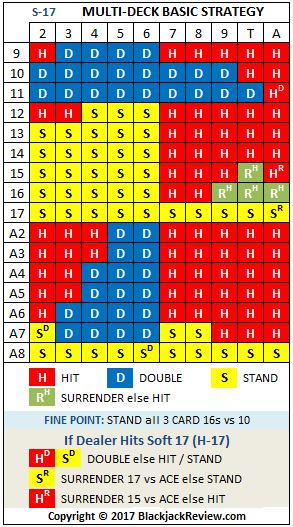
\includegraphics[scale=0.5,keepaspectratio]{figures/BasicStrategy_Multideck.jpg}
\end{center}
\caption{A Basic Strategy chart for multi-deck games}
\label{fig:BasicStrategy_Multideck}
\end{figure}

Figure \ref{fig:BasicStrategy_Multideck} illustrates the basic strategy for multi-deck Blackjack games. It provides the optimal action (Hit, Stand, Double, or Surrender) based on the player’s total hand value (listed on the left) and the dealer’s upcard (listed on the top). The actions are color-coded: red for Hit (H), yellow for Stand (S), blue for Double (D), and green for Surrender (R). Following this chart helps players make statistically optimal decisions, thereby minimizing the house edge and improving their chances of winning.

\vskip\baselineskip 
\textbf{General idea of basic strategy models are like this:}
\begin{itemize}
\item \textbf{Input Parameters:} The player's hand value and the dealer's upcard are taken as input parameters.
\item \textbf{Chart Lookup:} The model refers to the basic strategy chart to determine the optimal action for the given combination of the player's hand and the dealer's upcard.
\item \textbf{Decision Making:} Based on the chart's recommendation, the model decides whether to hit, stand, double down, or split.
\item \textbf{Execution:} The model executes the chosen action and updates the hand value accordingly.
\item \textbf{Iteration:} This process is repeated until the player's hand value indicates that no further actions are recommended (e.g., the player stands or busts).
\end{itemize}

\begin{figure}[H]
\framebox[6.0in]{
\begin{minipage}[b]{5.9in}
\begin{algorithmic}[1]
\REQUIRE player\_hand, dealer\_hand,deck
\STATE \textbf{Initialize} dealer\_up $\leftarrow$ dealer\_hand.cards[0]
\STATE \textbf{Initialize} action $\leftarrow$ find\_action(player\_hand, dealer\_up) in chart

\WHILE{True}
    \IF{action is Hit}
        \STATE Add a card from the deck to player\_hand
    \ELSIF{action is Double}
        \STATE Add another bet amount to table
        \STATE Add a card from the deck to player\_hand
        \STATE Leave the loop
    \ELSE
        \STATE Leave the loop
    \ENDIF
\ENDWHILE
\end{algorithmic}
\end{minipage}}
\caption{Basic Strategy gameplay loop}
\label{alg:stft}
\end{figure}

The find\_action function uses the player's hand value and the dealer's upcard to determine the next action by checking the basic\_strategy table in Figure \ref{fig:BasicStrategy_Multideck}. It retrieves and returns the optimal action for the current game state. In Figure \ref{fig:BasicStrategy_activitydiagram} we can see the activity diagram of basic strategy model:

\begin{figure}[htb]
\begin{center}
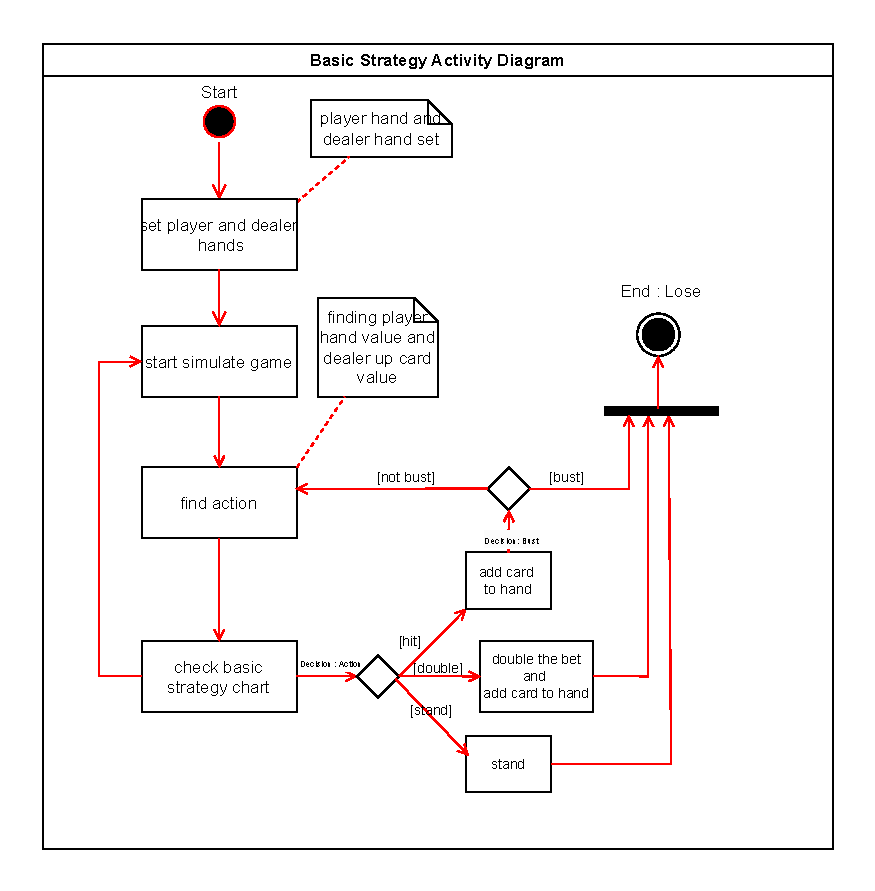
\includegraphics[scale=1,keepaspectratio]{figures/basic_strategy_activity_diagram.pdf}
\caption{Basic Strategy Activity Diagram} 
\label{fig:BasicStrategy_activitydiagram}
\end{center}
\end{figure}

The process starts with the initialization of hands for both the player and the dealer Than game simulation initiates based on these values, the appropriate action is identified by referring to a \textit{basic strategy chart}. If the player's hand has not busted, the player must choose between hitting, doubling, or standing. If the decision is to hit, an additional card is drawn and added to the player's hand. If the player opts to double, the bet is increased, an extra card is drawn, and the hand value is re-evaluated. Alternatively, if the decision is to stand, no further actions are taken, and the turn ends.This cycle continues until a final decision is made. If at any point the player's hand exceeds 21 (busts), the game concludes, and the player loses.

\subsection{Basic Strategy with Counting}
\label{basic_strateg_with_counting}
\textit{Card counting} is a technique used in Blackjack to track the ratio of high cards (10s, face cards, and Aces) to low cards (2 through 6) remaining in the deck. The underlying principle is that a deck with a higher proportion of high cards is advantageous for the player, as it increases the likelihood of achieving a natural Blackjack and improves the odds for doubli  ng down and splitting pairs. Conversely, a deck rich in low cards favors the dealer. Now let's look at how cart counting works:

\begin{itemize}
    \item \textbf{Assigning Values to Card} : Most counting techniques are using the system Hi-Lo as assigning values to cards.
    \begin{itemize}
        \item \textit{2 to 6} : + 1
        \item \textit{7 to 9} : 0
        \item \textit{10, Jack, Queen, King and Ace} : - 1
    \end{itemize}
    \item \textbf{Running Count} : As cards are dealt, the player keeps a running count by adding or subtracting the assigned values of each card that appears.
    \item \textbf{The True Count} : To account for the number of decks remaining, the player divides the running count by the estimated number of decks left to be dealt. This provides the "true count," which is a more accurate measure of the deck's favorability.
    \item \textbf{Adjuting the Bet} : The player adjusts their bets from the basic strategy based on the true count. Higher bets are placed when the true count is high (favorable deck), and certain strategy deviations (e.g., hitting, standing, doubling down) are made according to specific index plays derived from the true count.
\end{itemize}

While the basic strategy provides a set of optimal plays for given hands based on the dealer's upcard, card counting enhances this strategy by providing additional information about the composition of the remaining deck. In Figure \ref{alg:running_count}, Figure \ref{alg:update_running_count} and Figure \ref{alg:calcualte_true_count} we can see how to calculate running count, true count and adjusting the bet acording to these values.

\begin{figure}[H]
\framebox[6.0in]{
\begin{minipage}[b]{5.9in}
\begin{algorithmic}[1]
\REQUIRE card
\STATE \textbf{Initialize} card\_value $\leftarrow$ card.value
    \IF{card\_value in [2, 3, 4, 5, 6]}
        Increase count by 1
    \ELSIF{card\_value in [10, 11]}
        Decrease count by 1
    \ELSE
        Don't change count
    \ENDIF
\end{algorithmic}
\end{minipage}}
\caption{Counting cards}
\label{alg:running_count}
\end{figure}

In figure \ref{alg:running_count} we can see the part of \textit{Assigning Values to Card} part of the card counting strategy.

\begin{figure}[H]
\framebox[6.0in]{
\begin{minipage}[b]{5.9in}
\begin{algorithmic}[1]
\REQUIRE hand
\FOR{cards in hand}
\STATE \textbf{Initialize} runing\_count $\leftarrow$ runing\_count + count\_card(card)
\ENDFOR
\end{algorithmic}
\end{minipage}}
\caption{Update function for keeping the count of cards}
\label{alg:update_running_count}
\end{figure}

This function (Figure \ref{alg:update_running_count}) keeps the ruining count updated for each card dealt on the table. It is invoked whenever either the player or the dealer draws a card from the deck.

\begin{figure}[H]
\framebox[6.0in]{
\begin{minipage}[b]{5.9in}
\begin{algorithmic}[1]
\REQUIRE 
\STATE \textbf{Initialize} remaining\_decks $\leftarrow$ amount of remaining cards / 52
\STATE \textbf{Initialize} true\_count $\leftarrow$ runing\_count / remaining\_decks
\end{algorithmic}
\end{minipage}}
\caption{Function for calculating true count}
\label{alg:calcualte_true_count1}
\end{figure}

Finally, the function depicted in Figure \ref{alg:calcualte_true_count1} is essential for calculating the true count, which is a critical component of the card counting strategy. To minimize the house edge, the player must adjust their bet size based on the true count. This calculation helps determine the favorability of the remaining decks, thereby allowing the player to make more informed strategic decisions.

\begin{figure}[H]
\framebox[6.0in]{
\begin{minipage}[b]{5.9in}
\begin{algorithmic}[1]
\REQUIRE
\STATE bet\_multiplier $\leftarrow$ maximum of 1 and value of (true\_count multiplied by minimum of remaining\_decks and 1)
\STATE bet\_amount $\leftarrow$ self.minimum\_bet multiplied by bet\_multiplier
\RETURN minimum of bet\_amount and self.money
\end{algorithmic}
\end{minipage}}
\caption{Setting bet size acording to true count}
\label{alg:calculate_betsize}
\end{figure}

Using the true count, the player calculates a bet multiplier. This multiplier is determined as the maximum value between 1 and the product of the true count and the minimum of the remaining decks and 1. The bet amount is then calculated by multiplying the minimum bet with this bet multiplier. Finally, the bet amount is adjusted to ensure it does not exceed the player's available money.

After setting the bet size, the model continues to apply the basic strategy using the new bet size.

\subsection{Historical Data}
The Historical Data model leverages a large dataset of 50 million Blackjack hands \cite{url:1} to determine the optimal actions based on historical outcomes. This dataset, sourced from Kaggle, provides a comprehensive collection of simulated Blackjack hands, reflecting various scenarios and outcomes based on basic strategy. Due to the proprietary nature of casino data, this generated dataset serves as a valuable resource for analyzing and predicting optimal plays in Blackjack.

The dataset includes extensive information on each hand, such as cards remaining, dealer up, initial hand, dealer final, dealer final value, player final, player final value and actions taken. For our purposes, we focus on the columns that capture the initial hand, the dealer's up card, and the action taken. By analyzing these key elements, the Historical Data model can predict the best action for any given hand based on empirical evidence from millions of simulated plays.

The following pseudocode outlines the steps to process the dataset and determine the optimal action based on the initial hand and the dealer's upcard.

\begin{figure}[H]
\framebox[6.0in]{
\begin{minipage}{5.9in}
\begin{algorithmic}[1]
\REQUIRE key
\STATE query $\leftarrow$ "SELECT actions\_taken FROM historical\_data WHERE initial\_hand = ? AND dealer\_up = ? LIMIT 1"
\STATE result $\leftarrow$  Execute query with key[0] and key[1]
\IF{result exists}
    \RETURN result
\ELSE
    \STATE \textbf{USE BASIC STRATEGY}
\ENDIF

\RETURN most\_common\_action\_sequence
\end{algorithmic}
\end{minipage}}
\caption{Pseudocode for Check Next Move}
\label{alg:historical_data}
\end{figure}

As shown in Figure \ref{alg:historical_data}, a database query is created to find the current state in the Historical Data. If the exact game state (e.g., [5, 8] and 8) is found in the Historical Data, it checks for the most repeated action in the dataset and uses it. If it cannot find the exact state, it uses basic strategy to fill the gap in the Historical Data. The reason for using a SQL database in this case is that querying in a SQL database is faster than reading from a CSV file, which is crucial given the importance of speed in our scope.

\subsection{RL Model (Reinforcement Learning)}
\label{RL}
\textit{Reinforcement Learning (RL)} is a type of machine learning where an agent learns to make decisions by performing actions in an environment to maximize cumulative rewards. Unlike supervised learning, where the model learns from a dataset with labeled examples, RL involves learning through interaction with the environment, receiving feedback in the form of rewards or penalties, and using this feedback to improve future actions. The core idea is to develop a policy that dictates the best action to take in each state to achieve the highest long-term reward.

To create a model that uses reinforcement learning we need to complete some key steps:
\begin{itemize}
    \item \textbf{Defining Environment} : The environment in which the agent operates should be clearly defined, including the states, actions, and reward structure. In blackjack scope; agent is player, states are player's hand vs. dealer's up card, actions are hit and stand and double and rewarding is determined as winning or losing the current round of blackjack.
    \item \textbf{Initialization the Q-Table} : Q-Table is a table that stores the expected rewards for each state-action pair.
    \item \textbf{Choosing the Hyper-parameters} : Setting values like learning rate (alpha), discount factor (gamma) and exploration rate (epsilon).
    \item \textbf{Implementing a learning algorithm} : There are different learning algorithms differs in model-free RLs and model-based RL. They also splits in each category. In this project Q-learning algorithm from model-free algorithms will be used.
    \item \textbf{Training the model} : Running multiple episodes where the agent interacts with the environment and learns from the outcomes.
\end{itemize}

\subsubsection{Explanation of Q-Learning}
Q-learning is a reinforcement learning algorithm that aims to learn the value of the optimal action-selection policy. It uses a Q-Table to store the expected rewards for each state-action pair. The Q-learning algorithm updates the Q-Table based on the Bellman equation:

\begin{equation}
Q(s, a) \leftarrow Q(s, a) + \alpha \left[ r + \gamma \max_{a'} Q(s', a') - Q(s, a) \right]
\end{equation}
where:
\begin{itemize}
    \item $Q(s, a)$ is the current value of the state-action pair.
    \item $\alpha$ is the learning rate.
    \item $r$ is the reward received after taking action $a$.
    \item $\gamma$ is the discount factor.
    \item $s'$ is the next state.
    \item $\max_{a'} Q(s', a')$ is the maximum expected future reward for the next state-action pair.
\end{itemize}


Next, let's see how to implement Bellman's equation into the model training code in psudocode:

\begin{figure}[H]
\framebox[6.0in]{
\begin{minipage}{5.9in}
\begin{algorithmic}[1]
\FOR{each episode in range(num\_episodes)}
    \STATE state $\leftarrow$ reset()
    \STATE done $\leftarrow$ False
    
    \WHILE{not done}
        \IF{random number between 0 and 1 is less than epsilon}
            \STATE action $\leftarrow$ random choice from action\_space
        \ELSE
            \STATE action $\leftarrow$ index of the maximum value in q\_table[state]
        \ENDIF
        
        \STATE next\_state, reward, done, \_ $\leftarrow$ step(action)
        
        \IF{next\_state is not in q\_table}
            \STATE q\_table[next\_state] $\leftarrow$ [0, 0, 0]
        \ENDIF
        
        \STATE q\_table[state][action] $\leftarrow$ q\_table[state][action] + alpha * (reward + gamma * maximum value in q\_table[next\_state] - q\_table[state][action])
        
        \STATE state $\leftarrow$ next\_state
    \ENDWHILE
\ENDFOR
\end{algorithmic}
\end{minipage}}
\caption{Pseudocode for Train Model}
\label{alg:train_model}
\end{figure}

The train\_model function trains a reinforcement learning agent using the Q-learning algorithm over many episodes. Throughout the episode, the agent selects actions based on the current state using an epsilon-greedy policy, which balances exploration of new strategies and exploitation of known optimal actions. After performing an action, the environment provides feedback, including the next state, the reward, and whether the episode is complete. If the next state is new, it is added to the Q-table with initial Q-values. The Q-value for the current state-action pair is updated using the Bellman equation, incorporating the immediate reward and future reward estimates. This process allows the agent to iteratively improve its strategy, aiming to maximize long-term rewards.

\begin{figure}[htb]
\begin{center}
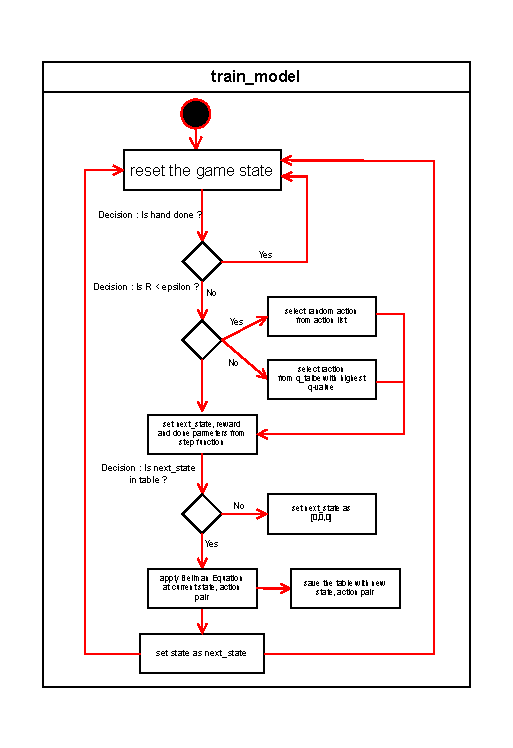
\includegraphics[scale=1.2,keepaspectratio]{figures/train_model_activitydiagram.pdf}
\end{center}
\caption{Train Model Activity Diagram}
\label{fig:train_model_activitydiagram}
\end{figure}

The Figure \ref{fig:train_model_activitydiagram} above illustrates the training process of the reinforcement learning (RL) model for the blackjack application. The process begins with resetting the game state to ensure a fresh start for each episode. The first decision checks if the hand is terminal, which determines if the episode should end. If not, the agent selects an action using an epsilon-greedy policy, balancing exploration and exploitation. Based on the chosen action, the game state is updated with the new card, and the environment provides feedback, including the next state and reward. The agent then updates the Q-value for the current state-action pair using the Bellman equation, incorporating both the immediate reward and the estimated future rewards. This cycle repeats until the hand is terminal, at which point the episode ends, and the game state is reset for the next episode.

\chapter{DESIGN AND IMPLEMENTATION}
\label{design-and-implementation}
The implementation of the algorithms for the models, user interface, and graphs are all written in Python. The majority of the algorithms utilize the Pandas library for handling data and saving the outputs of the simulations into Excel files for later analysis. For the Historical Data analysis model, SQLite is used to store .csv files into a local database, allowing for faster data searching compared to reading and searching within a .csv file directly. The reinforcement learning (RL) model employs the pickle library for serialization, enabling the saving of the Q-table to a file for future use in determining actions during the blackjack game. Graph creation within the user interface leverages the matplotlib and seaborn libraries, providing robust tools for data visualization. The entire graphical user interface (GUI) is developed using PyQt6, ensuring a rich and interactive user experience.

\section{User Interface}
This section discusses the user interface design, detailing the user interface elements, their functionality, and the benefits they provide to the user.
\vskip\baselineskip
\begin{figure}[htbp]
\begin{center}
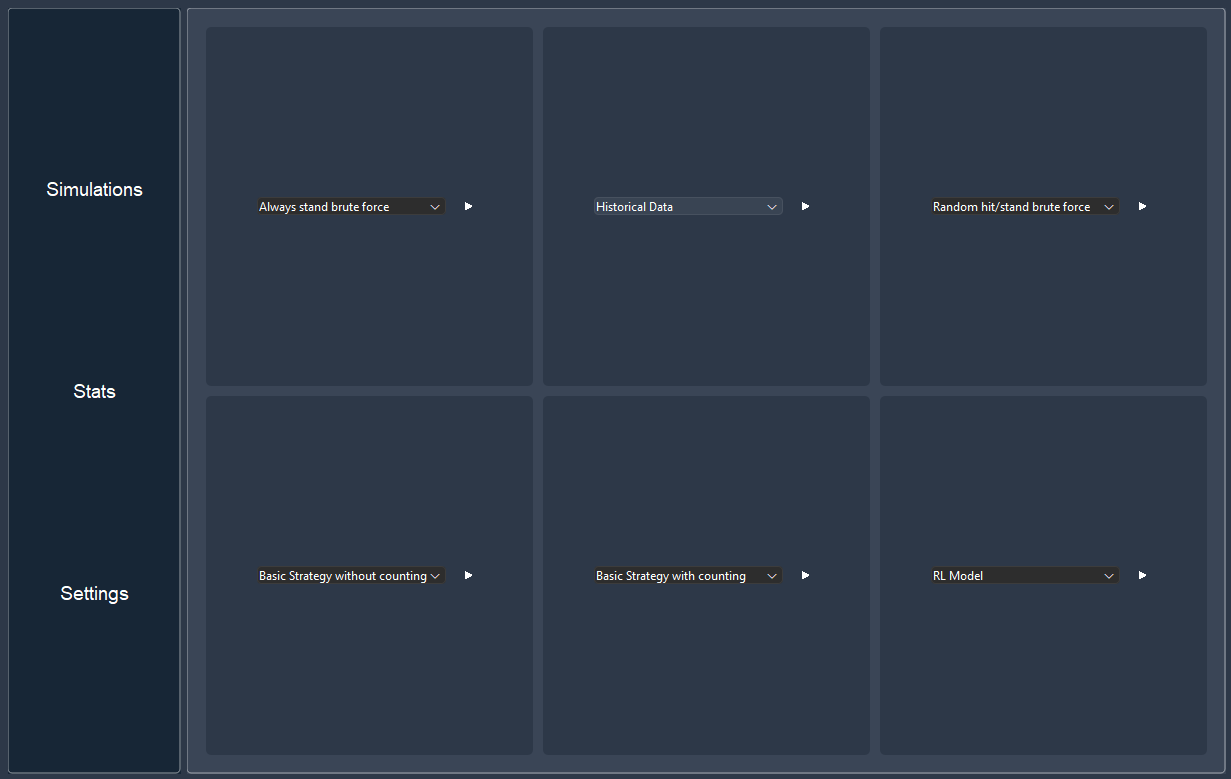
\includegraphics[scale=0.35]{simulation screen.png}
\end{center}
\caption{User Interface : Simulation Screen}
\label{fig:simulation_screen}
\end{figure}

In the simulation screen, users can select up to six models to run concurrently. After selecting the desired model names, pressing the "run" button will create a new thread for each model. The designated algorithms will then be simulated using default settings, unless specific settings have been configured by the user.

\vskip3\baselineskip
\begin{figure}[htbp]
\begin{center}
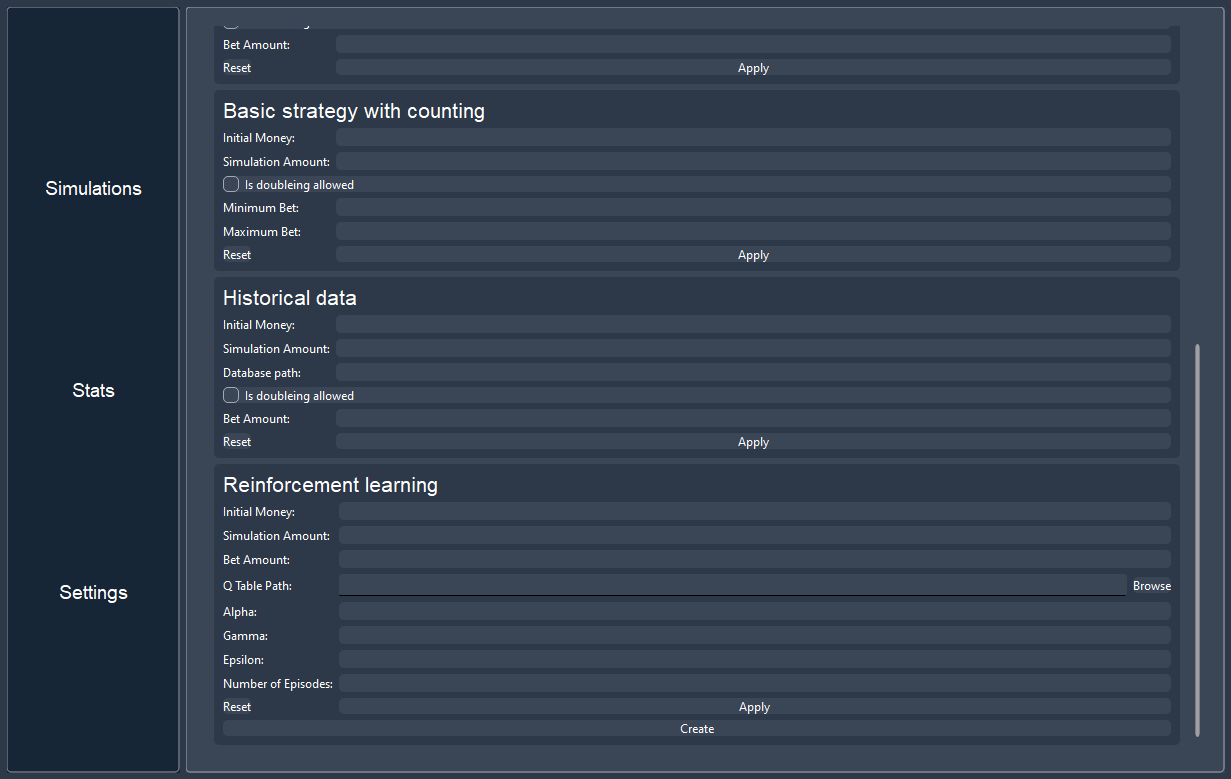
\includegraphics[scale=0.35]{settings screen.png}
\end{center}
\caption{User Interface : Settings Screen}
\label{fig:settings_screen}
\end{figure}

As mentioned above, simulations run with default settings by default. However, users can customize these settings as desired. Each model has different settings, in addition to common settings such as initial money, simulation amount, and bet amount. For example, as shown in \ref{fig:settings_screen}, the Reinforcement Learning model has numerous specific settings. These include simulation settings as well as parameters such as alpha, gamma, epsilon, and the number of episodes for training a model in real-time within the application. To simulate more customized models, users can adjust the desired variables from this settings screen.

\begin{figure}[htbp]
\begin{center}
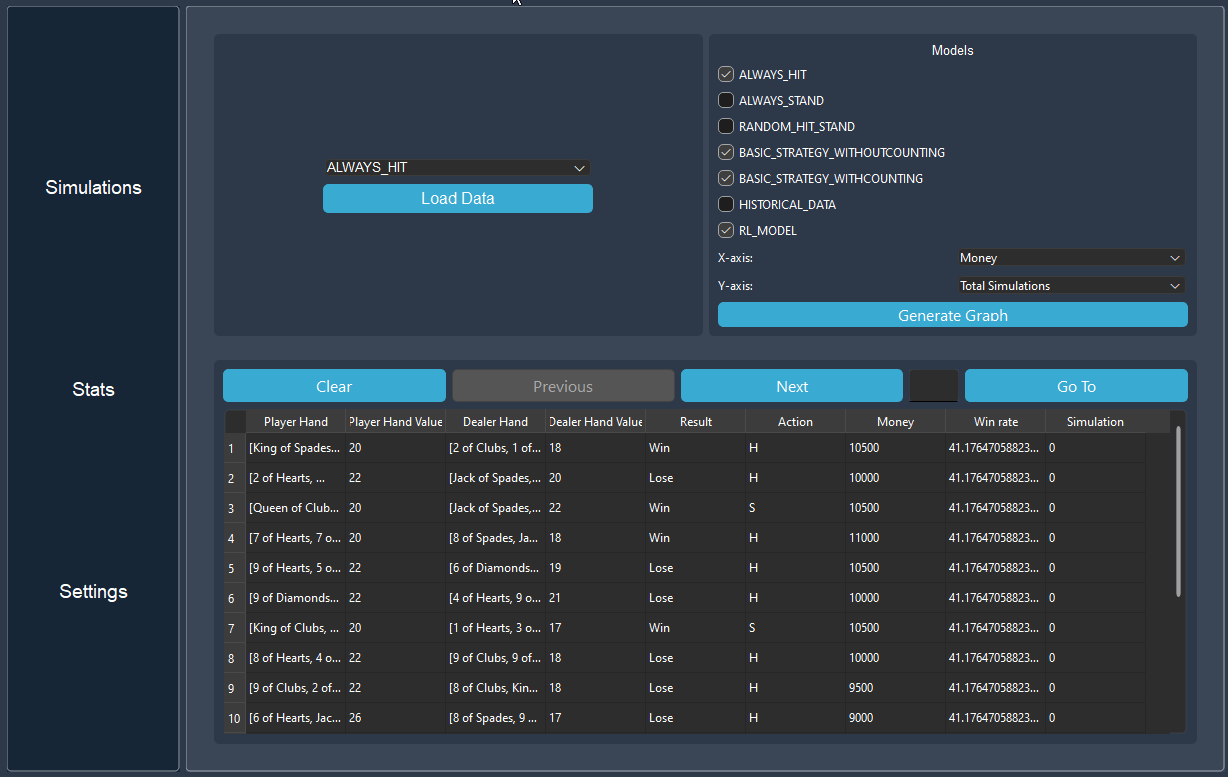
\includegraphics[scale=0.35]{stats screen.png}
\end{center}
\caption{User Interface : Stats Screen}
\label{fig:stats_screen}
\end{figure}

Once the simulations are run, the stats screen displays detailed results, including player hands, dealer hands, hand values, results, actions taken, and financial outcomes. Users can navigate through the simulation results, clear the data, and jump to specific simulations using the provided controls.

Additionally, the stats screen offers powerful visualization tools. Users can generate comparative graphs to analyze the performance of different algorithms, with customizable axes and parameters. Graphs are created using matplotlib and seaborn, providing clear and insightful visual representations of the data. This comprehensive analysis capability helps users identify the strengths and weaknesses of each algorithm, facilitating a deeper understanding and enabling the development of optimized blackjack strategies.

\chapter{TEST AND RESULTS}
\label{test-and-results}
In this chapter, the performance and efficacy of the created blackjack playing models will be rigorously compared across various scenarios and dimensions. Each model will be evaluated under different conditions to highlight their strengths and weaknesses. All the data presented in this chapter is directly derived from the application, ensuring accuracy and relevance. Comprehensive graphical representations will be provided for each model, allowing for a visual comparison of their performance. In addition, detailed tables will be included to facilitate an easier and more structured comparison of key metrics.

The analysis will cover several aspects, including win rates, loss rates, average monetary outcomes, and other relevant statistics. These comparisons will help in understanding how each model performs in different game situations, enabling a thorough evaluation of their effectiveness.

\section{Comparing Brute Force Models}
In this section, the brute force models—Always Hit, Always Stand, and Random Hit/Stand—will be compared in terms of win rate, loss rate, money change over win rate, and average return on investment for each model.


All the following algorithms are ran in these parameters:
\begin{itemize}
    \item Initial Money : 10000
    \item Simulation Amount : 2000
    \item Bet Amount : 500
    \item Hit/Stand Threshold (For always hit model) : 17 (by default)
\end{itemize}

\subsection{Always Hit}

The always hit brute force algorithm operates under a straightforward rule: it continues hitting until it reaches a specified threshold. Consequently, in some situations, this model may hit hands that should ideally be stood on, leading to sub-optimal game-play. In the next graph we will see the win rate over the 2000 simulations of always hit brute force model, then we will look into more performance oriented graph such as money x win rate and ROI.

\begin{figure}[h]
\begin{center}
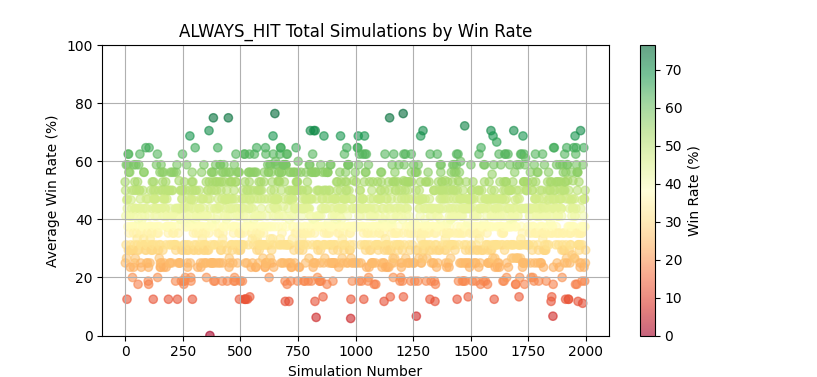
\includegraphics[scale=0.6]{figures/graphs/ah_wr_ts.png}
\end{center}
\caption{Always Hit Model : Win rate x Total Simulations}
\label{fig:ah_wr_ts}
\end{figure}

We observe a wide range of win rates, with some simulations achieving as high as 80\%, but many clustering around the 25-55\% range. This variability indicates that while the Always Hit strategy can occasionally perform well, it generally results in a moderate win rate, and there are some outliers at low 20's and high 80'. Now let's look at the money x win rate graph in order to get some intel about profitability of the model.

\begin{figure}[h]
\begin{center}
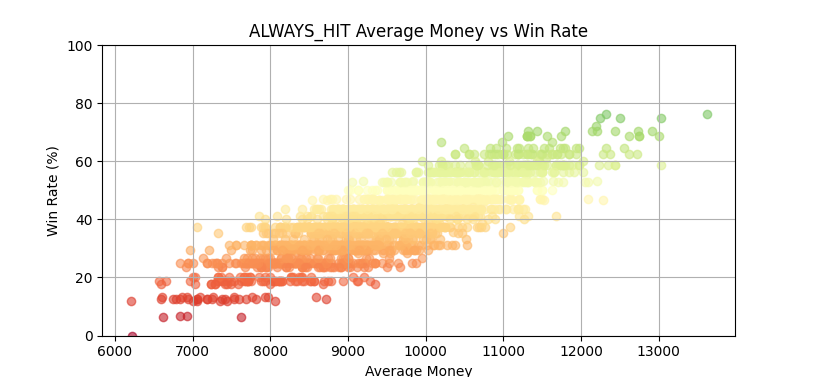
\includegraphics[scale=0.6]{figures/graphs/ah_money_wr_big.png}
\end{center}
\caption{Always Hit Model : Money x Win Rate}
\label{fig:ah_money_wr}
\end{figure}

The scarcity of data points on the right side indicates that the always hit model does not consistently guarantee a positive return on investment (ROI). However, within the win rate range of 50-80\%, the model shows a higher density of data points, suggesting that this is the zone where the model is more likely to be profitable. Now let's look at the ROI graph of this model to get better understanding in terms profitability.

\begin{figure}[h]
\begin{center}
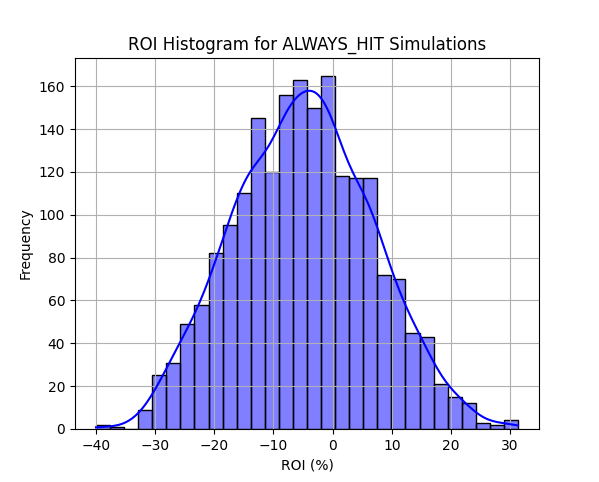
\includegraphics[scale=0.5]{figures/graphs/ah_roi.png}
\end{center}
\caption{Always Hit Model : ROI x Frequency}
\label{fig:ah_roi}
\end{figure}

As shown in Figure \ref{fig:ah_roi}, the graph peaks at an approximate average ROI of -5\%. Notably, the positive ROI section is in the minority, with only about 550 out of 1450 simulations achieving a positive return. This further indicates that the always hit model struggles to consistently generate profits.

Since we can set a threshold for the number until which the model will keep hitting, let's compare the thresholds of 16, 17, 18, and 19 with respect to each other:

\begin{figure}
    \begin{minipage}{0.45\textwidth}
        \centering
        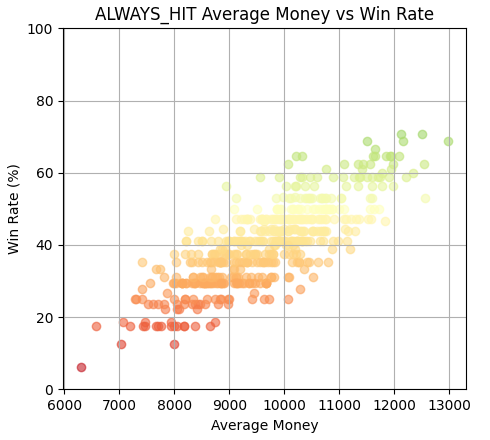
\includegraphics[scale=0.4]{figures/graphs/16.png}
        \label{fig:16}
    \end{minipage}
    \begin{minipage}{0.45\textwidth}
        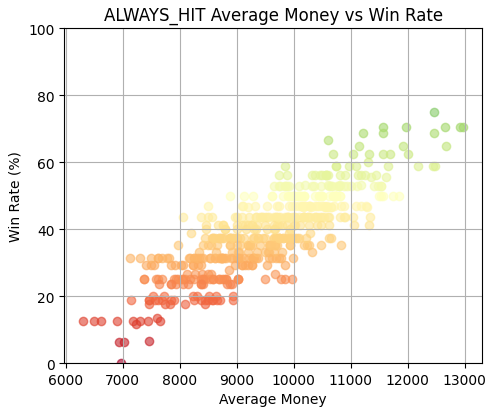
\includegraphics[scale=0.43]{figures/graphs/17.png}
        \label{fig:17}
    \end{minipage}
    \label{fig:16_17}
\end{figure}

\begin{figure}
    \begin{minipage}{0.45\textwidth}
        \centering
        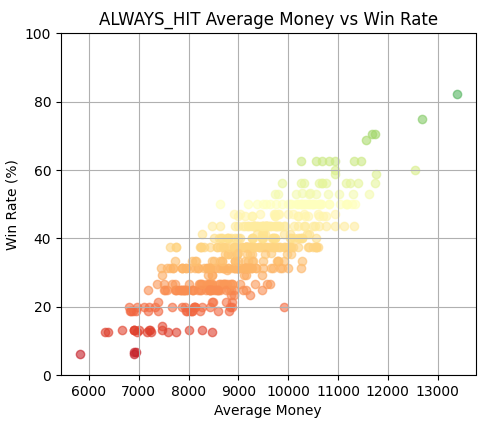
\includegraphics[scale=0.4]{figures/graphs/18.png}
        \label{fig:18}
    \end{minipage}
    \begin{minipage}{0.45\textwidth}
        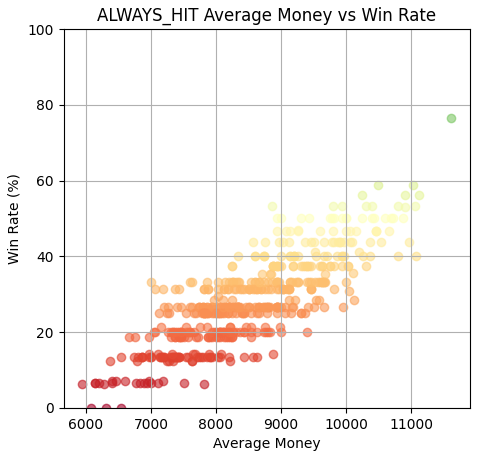
\includegraphics[scale=0.4]{figures/graphs/19.png}
        \label{fig:19}
    \end{minipage}
    \label{fig:18_19}
    \caption{Comprehension of always hit brute force model for thresholds 16, 17, 18 and 19}
\end{figure}

Here we can see that changing the threshold significantly impacts the behavior of the always hit brute force model. In the threshold 19 graph, win rates drastically drop to low 20\% values in many cases, with a limited spread in win rates. On the other hand, at threshold 16, while we observe fewer simulations, there is a notable decrease in win rates below 20\% compared to threshold 17. These graphs clearly show that the threshold setting has a substantial effect on the model's performance. Setting the threshold to 17 or 18 appears to be the most optimal approach, as indicated by the more favorable win rate distributions.


\subsection{Always Stand}
Since always stand model involves the computer standing  regardless of the total value of its hand. There may be performance and profitability since standing on a weak hand may generally lead to a lose. Below the graph of win rate x total simulations graph can be seen:

\begin{figure}[h]
\begin{center}
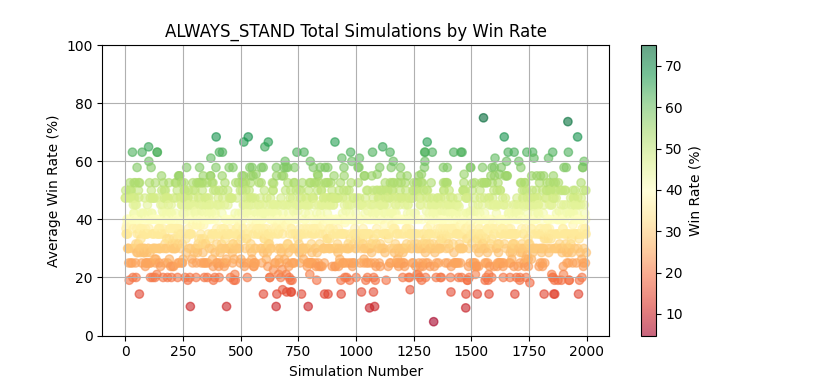
\includegraphics[scale=0.6]{figures/graphs/as_wr_ts.png}
\end{center}
\caption{Always Stand Model : Win rate x Total Simulations}
\label{fig:ah_wr_ts}
\end{figure}

Compared to the Always Hit model, the high win rate range is slightly lower, with the majority of simulations falling between 25-50\%, as opposed to 25-55\% for Always Hit. This indicates that the Always Stand strategy tends to perform less consistently at higher win rates, with fewer simulations achieving above 50\%. Now let's check Always Stand model's money x win rate graph to check its lucrativeness.

\begin{figure}[h]
\begin{center}
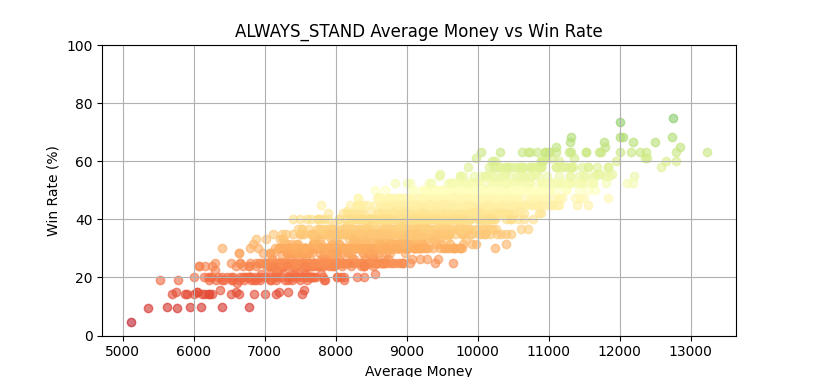
\includegraphics[scale=0.6]{figures/graphs/as_money_wr_big.png}
\end{center}
\caption{Always Stand Model : Money x Win Rate}
\label{fig:as_money_wr}
\end{figure}

Figure \ref{fig:as_money_wr} illustrates the performance of the Always Stand model. It is evident from the graph that the win rates above 60\% are disappeared. The majority of the data points fall within the 20-60\% win rate range, with only a small fraction of these achieving a profit. This indicates that the Always Stand model has limited profitability. We can also see this in ROI graph bellow:

\begin{figure}[h]
\begin{center}
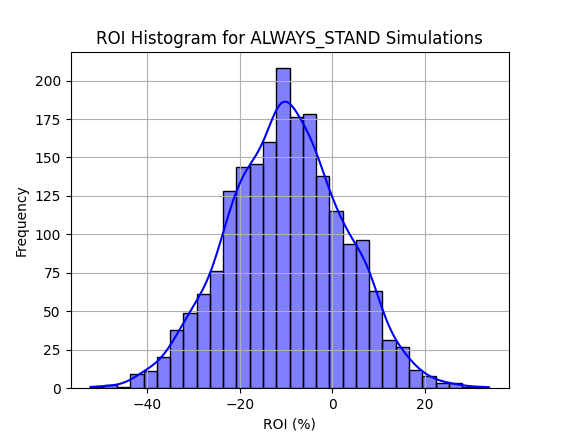
\includegraphics[scale=0.6]{figures/graphs/as_roi.png}
\end{center}
\caption{Always Stand Model : ROI x Frequency}
\label{fig:as_roi}
\end{figure}

Again, it is evident that the number of simulations with a positive ROI is drastically diminished. The ratio appears to be approximately 300 to 1700 in terms of +/- ROI's, indicating that the Always Stand strategy results in greater losses compared to the Always Hit strategy in blackjack.

So far, we have observed that always hitting outperforms always standing. Now, let's explore whether a random selection of actions (hitting or standing) might yield better results.

\subsection{Random Hit/Stand}
Since this approach simulates a more unpredictable style of play, which can sometimes  results in sub-optimal decisions, either hitting when it should stand or standing when it should hit. This variability may result in low performance in terms of ROI and money x win-rate. Let's first delve into the win rate x total simulations graph before mentioning money variable:

\begin{figure}[h]
\begin{center}
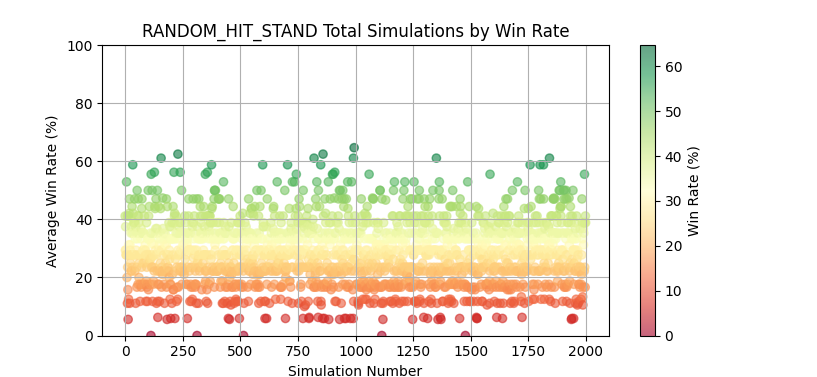
\includegraphics[scale=0.6]{figures/graphs/rhs_wr_ts.png}
\end{center}
\caption{Random Hit/Stand Model : Win rate x Total Simulations}
\label{fig:rhs_money_wr}
\end{figure}

Compared to the Always Hit and Always Stand models, the Random Hit/Stand strategy exhibits a less consistent performance. The win rates are more spread out, with a noticeable concentration in the 20-40\% range. The highest win rates achieved are slightly above 60\%, but the lower win rates extend down to around 10\%. This variability indicates that the Random Hit/Stand strategy is less reliable, with more simulations resulting in low win rates, and fewer achieving higher win rates. Now that we gathered information about win rates, lets dive into how this win rate effects profitability and ROI of the model:

\begin{figure}[h]
\begin{center}
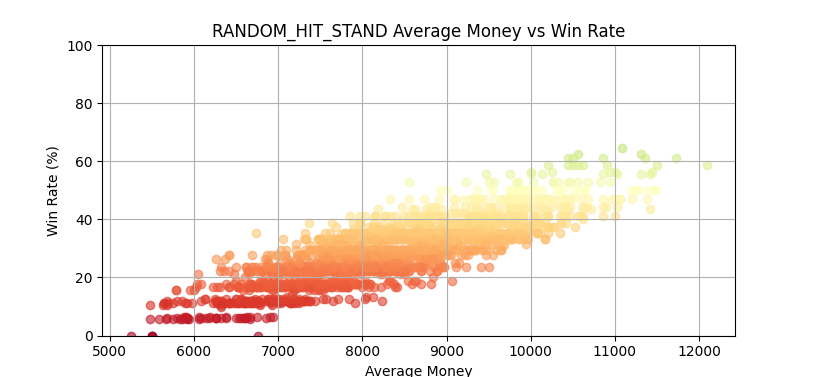
\includegraphics[scale=0.6]{figures/graphs/rhs_money_wr_big.png}
\end{center}
\caption{Random Hit/Stand Model : Money x Win Rate}
\label{fig:rhs_money_wr}
\end{figure}

As expected, selecting random actions results in worse outcomes compared to the other two models. The win rates for this model mostly fall below 55\%, with a significant number of games under 20\%. Given these results, it is clear that the ROI for this model is also lower than the others. Let's examine the ROI vs. Frequency graph to confirm this:

\begin{figure}[h]
\begin{center}
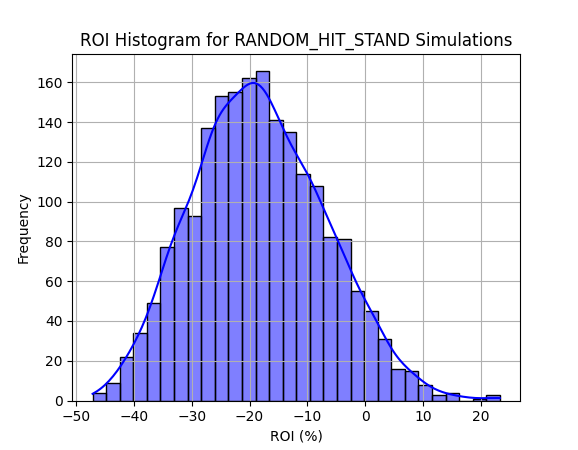
\includegraphics[scale=0.6]{figures/graphs/rhs_roi.png}
\end{center}
\caption{Random Hit/Stand Model : ROI x Frequency}
\label{fig:rhs_roi}
\end{figure}

The ROI has drastically diminished, with the ratio of positive to negative ROI being approximately 100 to 1900. This poor performance indicates that using a random action selection strategy in a normal game of blackjack is highly inadvisable. In fact, relying on any of the brute force models is generally unfavorable in terms of ROI. Therefore, let's set aside our "best" brute force model as Always Hit and proceed to evaluate presumably better models, such as those based on basic strategies.

\section{Comparing Basic Strategy Models}
In this section, we will compare the basic strategy without counting to the basic strategy with counting. Subsequently, we will evaluate the profitability of the better algorithm in comparison to our best brute force model, which is the Always Hit model.

\subsection{Basic Strategy without Counting}
As mentioned earlier in \ref{basic_strategy}, the basic strategy model determines its actions based on a \textit{basic strategy chart}. Let's first check that how well that basic strategy without counting performed in that 2000 simulation:

\begin{figure}[h]
\begin{center}
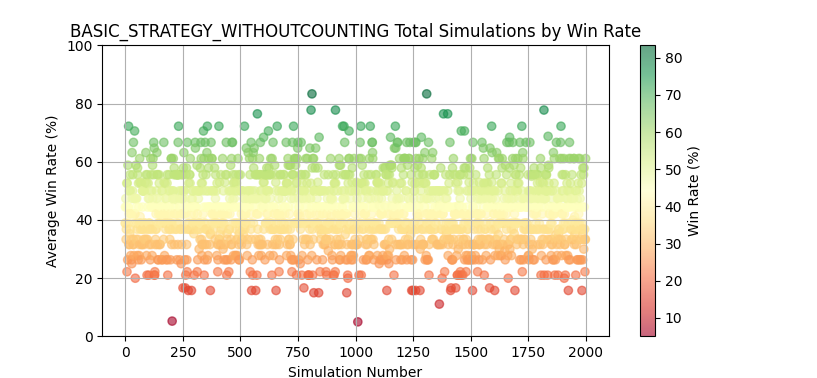
\includegraphics[scale=0.6]{figures/graphs/bswc_wr_ts.png}
\end{center}
\caption{Basic Strategy without Counting : Win rate x Total Simulations}
\label{fig:bswc_wr_ts}
\end{figure}

With respect to brute force models Basic Strategy without counting  shows a more concentrated distribution of win rates around 25-60\%. It performs quite like Always Hit model that we covered. But in basic strategy model that there are doubling involved in certain scenarios as a consequence of this this model may have more ROI in these cases. So let's examine the Money vs. Win Rate graph for the basic strategy model without counting to get better understanding in profitability of model:
 
\begin{figure}[h]
\begin{center}
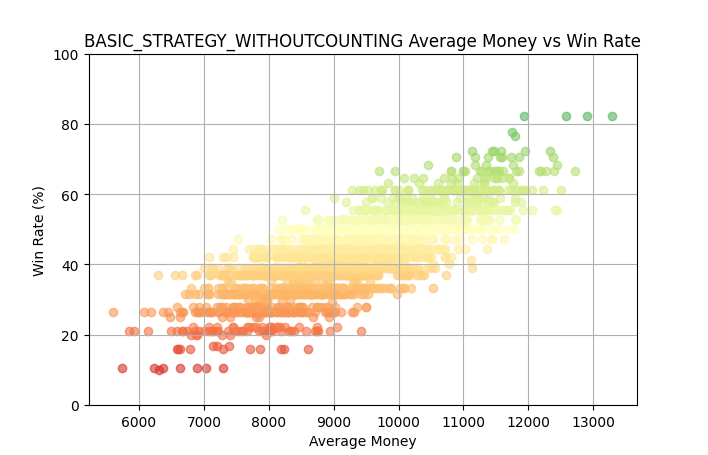
\includegraphics[scale=0.6]{figures/graphs/bswc_wr.png}
\end{center}
\caption{Basic Strategy without Counting : Money x Win Rate}
\label{fig:bswc_wr}
\end{figure}

In the graph, we observe that the basic strategy without counting resembles the Always Hit brute force graph but exhibits a higher maximum win rate and fewer low win rates. Although the majority of the games still fall on the unprofitable side, the basic strategy without counting performs almost as well as the Always Hit brute force model.

Let's now examine the ROI graph of the basic strategy without counting and compare it side by side with the Always Hit model. This comparison will provide a better understanding of the differences in their performance and profitability.

\begin{figure}
    \begin{minipage}{0.45\textwidth}
        \centering
        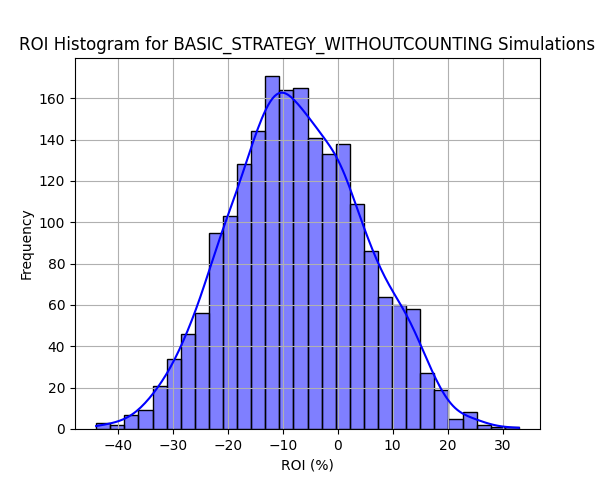
\includegraphics[scale=0.4]{figures/graphs/bswc_roi.png}
        \label{fig:ah_roi_left}
    \end{minipage}
    \begin{minipage}{0.45\textwidth}
        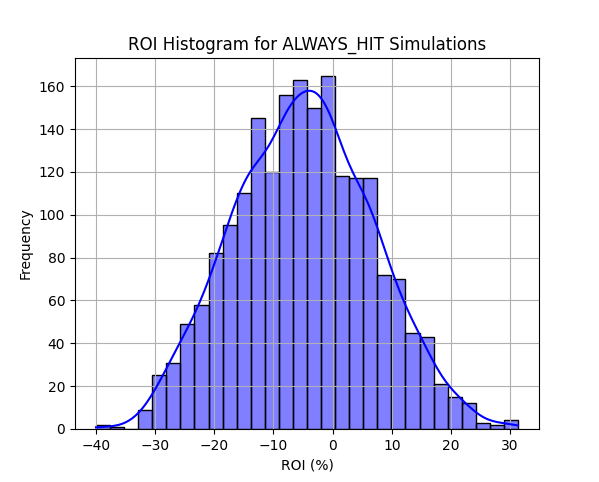
\includegraphics[scale=0.4]{figures/graphs/ah_roi.png}
        \label{fig:bswc_roi_right}
    \end{minipage}
    \label{fig:comparison_roi}
    \caption{Comparison between Basic Strategy without counting and Always hit model}
\end{figure}

We observe that there is not a significant difference in ROIs between these models. In the basic strategy model, the 0-5\% ROI range is slightly steeper means that it has more neutural like ROIs compared to the Always Hit model, but the average ROI for both models is approximately the same.

\subsection{Basic Strategy with Counting}

In \ref{basic_strateg_with_counting}, we discussed the basic strategy with counting. The counting method is used in blackjack to adjust bets according to the calculated house edge in the current situation. By counting high and low cards and dividing by the remaining decks, we obtain the true count, which is then used to set the bet size.

Since adjusting bets is a fundamental aspect of this model, there are several situations that we might encounter. 

True count may increase a lot due to cards in the deck are nearing to end bet size can be increase in unwanted ways. In order to prevent this maximum bet in settings should be set advisedly. Even though a maximum bet size is set, the algorithm may still incur significant losses as the end of the deck approaches. This situation can arise because the true count can become highly volatile with fewer remaining cards, leading to larger swings in betting amounts and potential losses.

First, let's evaluate the performance of the basic strategy with counting in terms of win rate x total simualtions done:

\begin{figure}[h]
\begin{center}
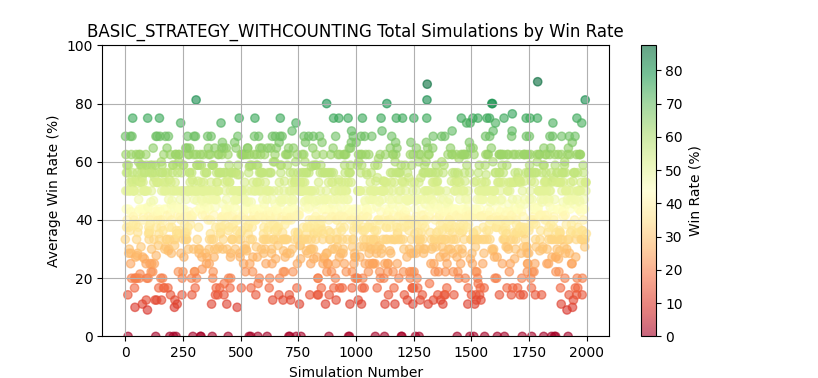
\includegraphics[scale=0.6]{figures/graphs/bsc_wr_ts.png}
\end{center}
\caption{Basic Strategy with Counting : Win rate x Total Simulations}
\label{fig:bsc_wr_ts}
\end{figure}

Graph for the Basic Strategy With Counting model presents a more intriguing pattern compared to the other strategies. As mentioned above, model may act more unstable with respect to other models so this results in a noticeable presence of outliers, with some simulations showing win rates near 0\% (or 0), while others exhibit exceptionally high win rates. This variability indicates that while the counting strategy can lead to substantial gains under favorable conditions, it also introduces a higher risk of significant losses when the true count leads to larger bets. Bellow is the Money x Win rate graph of basic strategy with counting model, let's check how the unstability of the model effects money x win rate and ROI graphs.

\begin{figure}[h]
\begin{center}
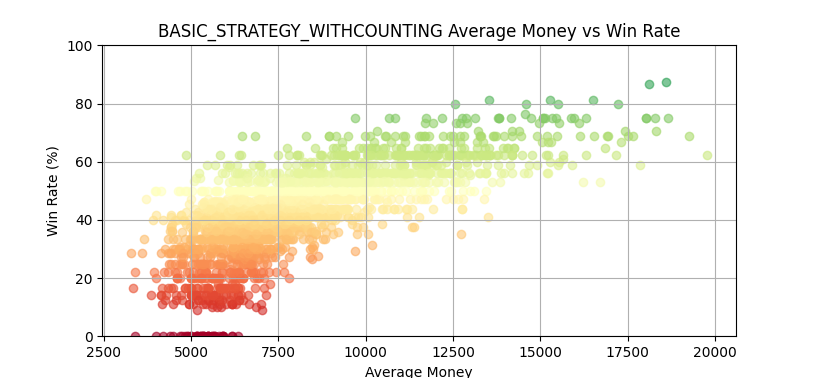
\includegraphics[scale=0.6]{figures/graphs/bsc_money_wr_big.png}
\end{center}
\caption{Basic Strategy with Counting : Money x Win Rate}
\label{fig:bsc_wr}
\end{figure}

At first glance, it is evident that there is a significantly higher number of simulations with win rates above 50\% in the graph. The money axis is also wider, indicating that the counting technique allows the model to win more money by increasing bets when favorable conditions are detected. However, we also observe a considerable number of simulations with win rates in the 0-20\% range. This is due to the previously mentioned reason: when the true count becomes very high, the algorithm starts to bet excessively, which can lead to the player going bankrupt.

But aside from the losing cases ROI of this model may be higher than the others, because of the risking factor of the model. Lets see ROI table of it next:

\begin{figure}[h]
\begin{center}
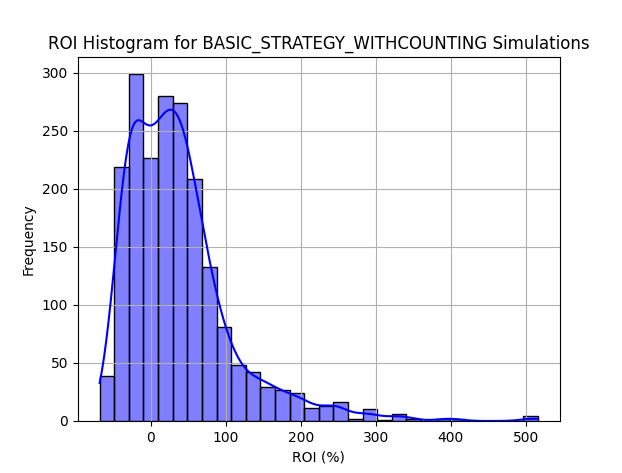
\includegraphics[scale=0.5]{figures/graphs/bsc_roi.png}
\end{center}
\caption{Basic Strategy without Counting : ROI x Frequencies}
\label{fig:bsc_roi}
\end{figure}

As clearly shown in Figure \ref{fig:bsc_roi}, the ROI of the basic strategy with counting model is significantly higher than the models we have discussed so far. The risk factor plays a crucial role here, as mentioned earlier. Playing with larger bets comes with greater responsibilities and potential for significant losses.

\section{Comparing Historical Data Model}
This method uses a database of past blackjack hands to inform decision-making, allowing the model to choose actions based on historical outcomes in similar situations. By leveraging this data, the model aims to mimic the decisions that have previously led to favorable results.

The model may face limitations if the Historical Data does not adequately cover all possible game situations. In that case model is going to use basic strategy as we mentioned before.

Despite these challenges, the Historical Data model can offer significant advantages by using empirical evidence to guide decision-making. Let's check that how Historical Data performs in terms of win rate over simulations:

\begin{figure}[h]
\begin{center}
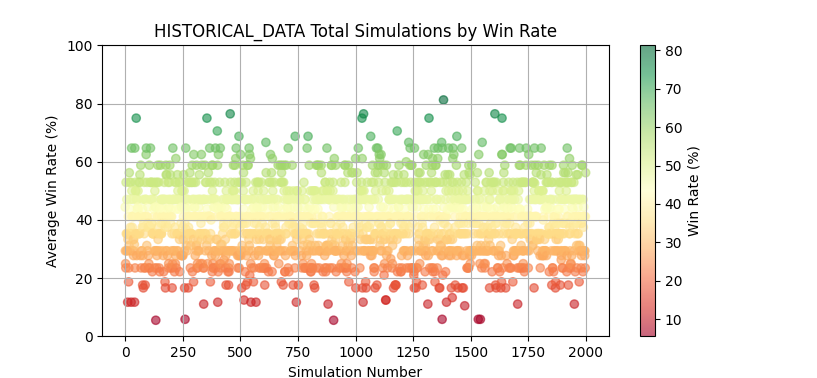
\includegraphics[scale=0.6]{figures/graphs/hd_wr_ts.png}
\end{center}
\caption{Historical Data : Win rate x Total Simulations}
\label{fig:hd_wr_ts}
\end{figure}

The graph for the Historical Data model indicates a distribution of win rates that closely resembles that of the Basic Strategy without Counting model. The win rates generally fall within the 20-50\% range, with a moderate number of simulations achieving win rates above 50\%. 

This similarity arises because the Historical Data model frequently resorts to basic strategy in the absence of sufficient Historical Data for specific scenarios. Consequently, the performance of the Historical Data model is highly dependent on the quality and coverage of the Historical Data. In simulations where the Historical Data is sparse or non-representative, the model defaults to basic strategy, resulting in win rates and performance metrics that align closely with those of the basic strategy without counting. Below is the Money x Win Rate graph of the Historical Data model:

\begin{figure}[h]
\begin{center}
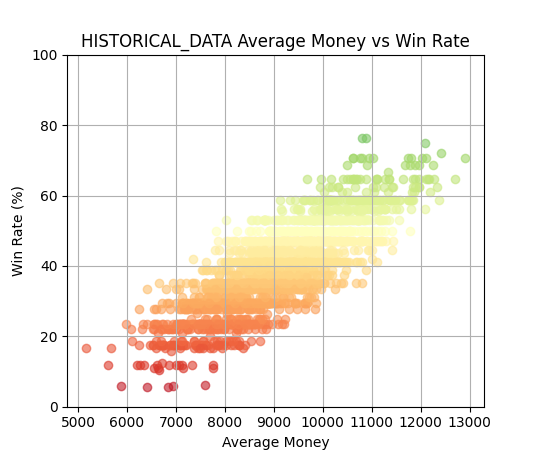
\includegraphics[scale=0.6]{figures/graphs/hd_wr.png}
\end{center}
\caption{Historical Data Model: Money x Win Rate}
\label{fig:hd_wr}
\end{figure}

As we can infer from the graph, the Historical Data model does not perform as well as the basic strategy with counting. Its performance is approximately the same as the Always Hit model and the basic strategy without counting. One reason for this could be the nature of the Historical Data. In the 2000 games simulated, there may have been scenarios where the specific Historical Data was less applicable, causing the algorithm to default to the basic strategy. In fact, the ratio of calling the basic strategy within the 50 million hands dataset was 40\%. Therefore, it is normal for this model to resemble the basic strategy without counting.

In another set of 2000 simulations, the odds could be more favorable, and more historically accurate data could be used, potentially increasing the win rate. Conversely, the opposite could also occur, leading to a lower win rate.

Now, let's examine the ROI graph for the Historical Data model to better understand its profitability:

\begin{figure}[h]
\begin{center}
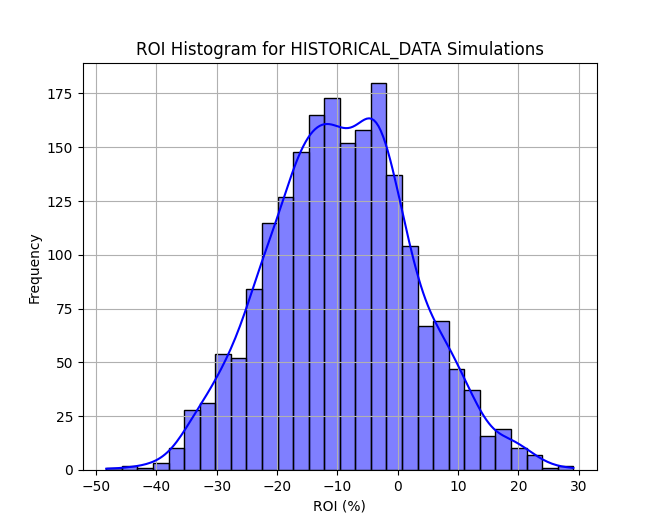
\includegraphics[scale=0.5]{figures/graphs/hd_roi.png}
\end{center}
\caption{Historical Data Model: ROI x Frequencies}
\label{fig:hd_roi}
\end{figure}

As mentioned it doesn't have a viable ROI to use this model in blackjack games. In this 2000 simulations it has even lower ROI average then always hit model, which is a brute force model.

\section{Comparing RL (Reinforcement Learning) Model}

As mentioned in Chapter \ref{RL}, reinforcement learning (RL) is a sophisticated machine learning model that utilizes a learning algorithm, specifically Q-Learning in this instance, to make decisions and perform actions within an environment to maximize the "reward." In our application, we first create and train the RL model using various parameters. This pre-trained model is then used to simulate games, leveraging its learned experience to make optimized decisions. Unlike the other models we've discussed, which rely on fixed rules or Historical Data, the RL model continuously learns and evolves during its training phase, enabling it to make more informed and optimized decisions when applied in the game simulations. Given its extensive learning process and adaptability, we anticipate that the RL model will outperform the other models in terms of efficiency and profitability. 

Before delving into money x win rate and ROI graphincs lets first look at how well RL model will perform in terms of win rate x total simulations:

\begin{figure}[h]
\begin{center}
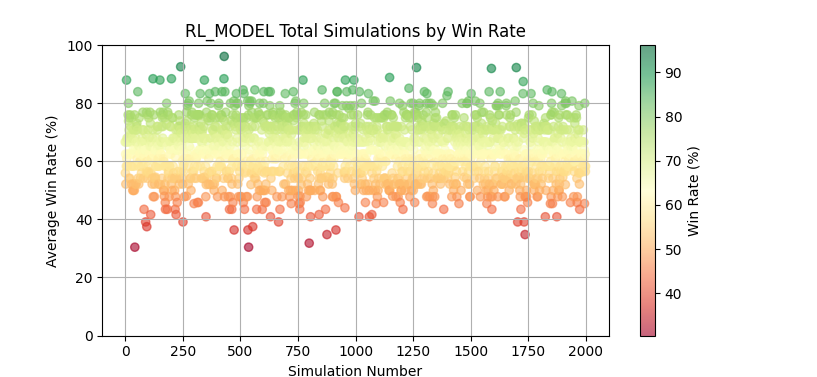
\includegraphics[scale=0.6]{figures/graphs/rl_wr_ts.png}
\end{center}
\caption{Historical Data : Win rate x Total Simulations}
\label{fig:rl_wr_ts}
\end{figure}

The graph for the Reinforcement Learning (RL) model shows a higher overall win rate compared to other models. Most simulations achieve win rates in the 50-80\% range, with several exceeding 80\%. This indicates the RL model's superior learning capability and adaptability in optimizing decisions. The RL model consistently performs well, as reflected by the tight clustering of win rates around the higher percentages. This consistency and higher win rate make the RL model a promising approach for blackjack strategies. Now lets look at Money X Win Rate graph of Reinforcement Learning model in order to get more visual information about the models success:
\vskip\baselineskip

\begin{figure}[h]
\begin{center}
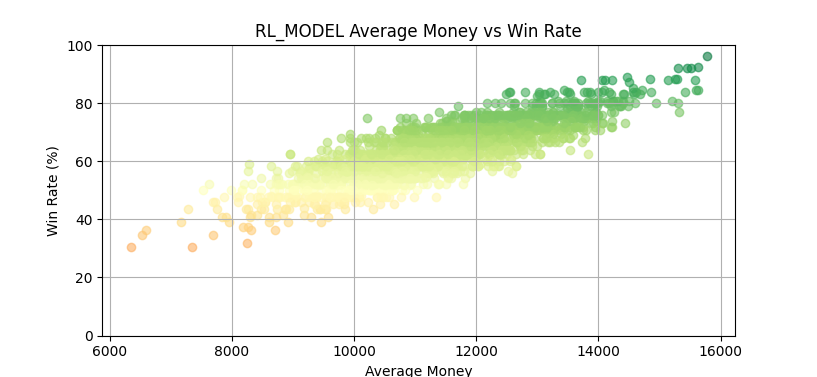
\includegraphics[scale=0.6]{figures/graphs/rl_money_wr_big.png}
\end{center}
\caption{Reinforcement Learning: Money x Win Rate}
\label{fig:rl_wr}
\end{figure}

\vskip\baselineskip

We can clearly see that the RL model achieves significantly higher profitability compared to the other models. Remarkably, there are approximately 100 simulations with a win rate exceeding 80\%, as will be further illustrated in the ROI chart discussed next. On average, the majority of the simulations fall within the 55-65\% win rate range, which is still superior to any of the previously examined models. To ensure that these results are not merely due to favorable training conditions, we will generate additional charts with 2000 simulations at the end of this chapter to verify the consistency and reliability of the model's performance.

Let's now examine the ROI table to assess the consistency of the RL model in terms of returning the player's investment in the game:

\begin{figure}[h]
\begin{center}
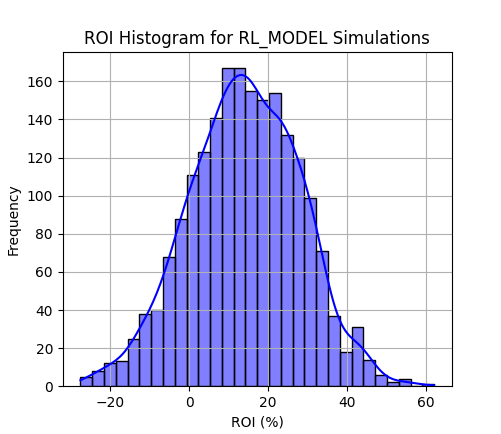
\includegraphics[scale=0.5]{figures/graphs/rl_roi.png}
\end{center}
\caption{Reinforcement Learning: ROI x Frequencies}
\label{fig:rl_roi}
\end{figure}

As shown in the figure \ref{fig:rl_roi}, demonstrates a notable consistency in the model's ability to return the player's investment. The majority of the simulations fall within the 0-30\% ROI range, with a prominent peak around the 15-20\% mark. This indicates that most of the simulations are profitable, providing a positive return on investment.


\begin{figure}[h]
    \begin{minipage}{0.45\textwidth}
        \centering
        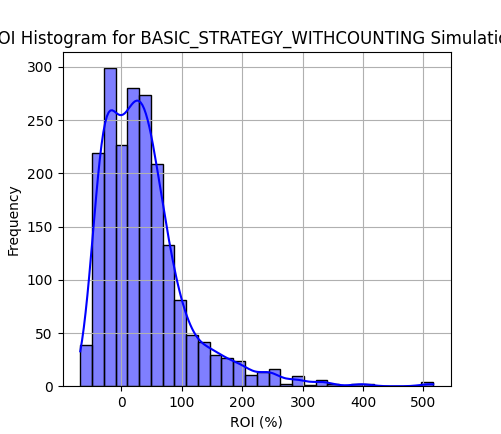
\includegraphics[scale=0.5]{figures/graphs/rl_vs_bsc_roi1.png}
        \label{fig:ah_roi_left}
    \end{minipage}
    \begin{minipage}{0.45\textwidth}
        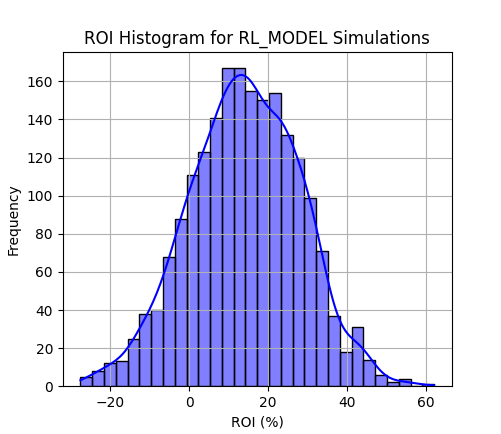
\includegraphics[scale=0.5]{figures/graphs/rl_roi.png}
        \label{fig:bswc_roi_right}
    \end{minipage}
\label{fig:comparison_roi}
\caption{Comparison between Basic Strategy with counting and Reinforcement Learning}
\end{figure}

In Figure \ref{fig:comparison_roi}, we compare our best ROI models that we gone trough. If we first check it by just the shape of it we can see that basic strategy without counting has more skewed graph, that has its peeks at -10-10\%'s with extending its ROI up to 500\% in some simulations which we can categorize them as outliers. On the other hand RL model histogram has much more symmetrical and bell-shaped graph, which suggests us that the RL model provides more consistent returns, with fewer extreme outliers.

The RL model has a small portion of simulations with negative ROI, but these are relatively few and less severe, mostly ranging between -20\% and 0\%. This indicates that the RL model has a lower risk of significant losses. On the contrary basic strategy with counting model, have negative ROI in graph (reaching from -40 to 0), might still present a risk due to the high variability in its returns, as indicated by the long positive tail.

The RL model demonstrates greater consistency and predictability in its performance. The narrow spread of ROI values around the peak indicates that simulations yield a similar range of returns, making it a more reliable model for consistent gains. But in basic strategy without counting with its wider spread and occasional high returns, suggests that while it can achieve very high returns in certain scenarios, it is less predictable and carries a higher variance in outcomes.

Overall, the RL model outperforms the both next best performed model basic strategy with counting model and the other models in terms of consistency and predictability, providing a more reliable and steady return on investment. The Basic Strategy with Counting model, while capable of achieving very high returns in some cases, exhibits greater variability and higher risk. 

\chapter{CONCLUSION}
\label{chapter:conclusion}

The comparative analysis of various blackjack strategies provides valuable insights into their performance and profitability. 

The brute force methods, including always hit, always stand, and random hit/stand, show fundamental differences in their win rates and ROI. Among these, the always hit strategy demonstrates the best performance, when its hit threshold set wisely, though it remains sub-optimal compared to more sophisticated models.

Basic strategy models, both with and without card counting, offer significant improvements over brute force methods. The basic strategy with counting model, shows higher win rates and potential for larger profits due to its adaptive betting strategy. However, this model also exhibits greater volatility, with notable outliers due to its aggressive betting behavior when the true count is high. The over-betting situation is also can be solved via setting a reasonable maximum bet size.

The reinforcement learning (RL) model stands out as the most consistent and profitable strategy. Trained using a variety of hyper-parameters, the RL model not only achieves high win rates but also maintains a balanced ROI across simulations. This consistency makes it a reliable choice for players seeking stable returns.

Historical data models, while informative, do not perform as well as the RL and counting strategies. Their reliance on past data leads to mixed results, with performance heavily dependent on the specific dataset used.

In summary, while the basic strategy with counting can achieve high returns in certain conditions, the reinforcement learning model proves to be the most effective overall, offering a balance of high win rates and consistent ROI. Further optimization of hyper-parameters could enhance the RL model's performance even more, solidifying its position as the best strategy for blackjack gameplay.

\section{Future Work}
Several enhancements and extensions can be implemented to improve the current system and provide a more comprehensive analysis of blackjack strategies:

\begin{itemize}
    \item {\textbf{User Interface Improvements:}} The GUI can be made more user-friendly and responsive, offering better feedback to users. For instance, incorporating sounds to notify users when simulations are complete would enhance the user experience.

    \item {\textbf{Graph Performance Optimization:}} The current graph creation screen can be slow when handling large datasets. For example, creating a graph with 2000 simulations, each with approximately 30 games, results in processing around 60,000 games, which can cause lag. Developing a custom graphing system could mitigate these performance issues.
    
    \item {Expansion of Brute Force Models:} New brute force models, such as "always doubling" or "imitate dealer" \cite{} THERE WILL BE CITE can be added to the system. Alternatively, these strategies can be integrated into existing models to provide a broader range of simulation options.
    
    \item {\textbf{Enhancements to Basic Strategy Models:}} Implementing features like insurance and surrendering could offer a more complete basic strategy model. Although these features may not significantly impact the results in 2000 simulations, their inclusion would provide a more accurate representation of real gameplay. Additionally, different counting strategies beyond the HI-LO \cite THERE WILL BE OTHER COUNTING STRATEGIES CITED method could be used, offering users the ability to select and compare various counting methods through the settings.
    
    \item {\textbf{Improvement of Historical Data Models:}} Access to better historical data would significantly enhance the accuracy and reliability of the historical data model. However, due to the restrictive nature of casinos regarding this information, obtaining such data may be challenging. If viable methods to access more comprehensive historical data are found, they should be increase the performance of the model.
    
    \item {\textbf{Advancements in Reinforcement Learning Models:}} The RL model can be further refined by incorporating additional actions, beyond just hit, stand, and doubling. Exploring other RL algorithms and comparing their performance could yield valuable insights. Additionally, a real-time learning model that updates based on the current data during gameplay could be developed.
\end{itemize}


\printbibliography

\appendix
\chapter{RUST CODE}

\fontsize{8}{8}\selectfont
\begin{verbatim}
//lib.rs

#![feature(step_by)]
#![allow(dead_code)]
#![allow(deprecated)]
#![feature(use_extern_macros)]

extern crate hound;
extern crate arrayfire;

use arrayfire::{Array, Dim4, Seq};

use std::f64;
use std::os::raw;
use std::ffi::CString;
use std::path::Path;
use std::slice;

mod spectrogram;
mod filters;
mod postprocess;

#[repr(C)]
pub struct FFI_Spectrogram {
    data : *const *const raw::c_double,
    shape : (u64, u64),
}

#[no_mangle]
pub fn analyze(file_name: *const raw::c_char, window_size: raw::c_uint, highpass: raw::c_uint, 
               hps_rate: raw::c_uint) -> *const *const raw::c_void
{
    //println!("Active Backend: {}", arrayfire::get_active_backend());
    
    println!("reading file...");
    let name: String = unsafe{std::ffi::CStr::from_ptr(file_name)}.to_string_lossy().into_owned();
    let mut reader = hound::WavReader::open(name.clone()).unwrap();

    //print_audio_details(&reader);

    let data : Vec<f64> = reader.samples::<i16>().map(|sample| sample.unwrap() as f64).collect();
    let mut data_af = Array::new(&data, Dim4::new(&[data.len() as u64,1,1,1])); 
  
    println!("applying preprocess filters..."); // TODO: filters as parameters
    data_af = ::filters::highpass(data_af, highpass as usize);
    //data_af = ::filters::lowpass(data_af, 330);

    let mut graphs = Vec::<*const raw::c_void>::new();        

    println!("calculating narrowband spectrogram...");
    let window_size = (2. as f64).powi(window_size as i32) as usize;
    let complex = spectrogram::stft(&data_af, window_size, 1024);
    let narrowband = spectrogram::complex_to_magnitude(&complex);
    graphs.push(to_ffi(&spectrogram::to_host(&narrowband)));
    
    println!("calculating wideband spectrogram...");
    let wideband = spectrogram::get_spectrogram(&data_af, 44100, 1024);
    graphs.push(to_ffi(&spectrogram::to_host(&wideband)));

    println!("combining spectrograms...");
    let combined = spectrogram::combine(&narrowband, &wideband);
    graphs.push(to_ffi(&spectrogram::to_host(&combined)));    

    println!("calculating harmonic product spectrum...");
    let hps = spectrogram::harmonic_product_spectrum(combined, hps_rate);
    graphs.push(to_ffi(&spectrogram::to_host(&hps)));    

    println!("getting frequencies...");
    let frequencies = spectrogram::get_frequencies(&hps);
    let mut frequencies_host : Vec<raw::c_uint> = vec![0; frequencies.elements()];
    frequencies.host(frequencies_host.as_mut_slice());
    let freq_p = Box::into_raw(frequencies_host.into_boxed_slice()) as *const raw::c_uint;
    graphs.push(freq_p as *const raw::c_void);

    println!("onset detection function...");
    let phase = spectrogram::complex_to_phase(&complex);
    let complex_df = spectrogram::onset_detection(&narrowband, &phase);
    let detect_p = Box::into_raw(complex_df.into_boxed_slice()) as *const raw::c_double;
    graphs.push(detect_p as *const raw::c_void);

    println!("Analysis completed.");    
    arrayfire::device_gc();

    Box::into_raw(graphs.into_boxed_slice()) as *const *const raw::c_void
}

fn to_ffi(s : &Vec<Vec<f64>>) -> *const raw::c_void
{
    let p_array : Vec<*const raw::c_double> = 
        s.iter().map(|c| Box::into_raw(c.clone().into_boxed_slice()) as *const raw::c_double).collect();
        
    let spect = FFI_Spectrogram {
        shape : (s.len() as u64, s[0].len() as u64),
        data : Box::into_raw(p_array.into_boxed_slice()) as *const *const raw::c_double
    };

    Box::into_raw(Box::new(spect)) as *const raw::c_void
}

fn post_filter(spectrogram: &Array, above: usize, below: usize) -> Array
{
    let sequence0 = Seq::new(above as u32, below as u32, 1);
    let sequence1 = Seq::new(0, (spectrogram.dims()[1]-1) as u32, 1);
    let mut idxr = arrayfire::Indexer::new();            
    idxr.set_index(&sequence0, 0, Some(true));
    idxr.set_index(&sequence1, 1, Some(true));    
  
    arrayfire::index_gen(&spectrogram, idxr)
}

#[no_mangle]
pub extern fn clean2d( ptr : *const raw::c_void) 
{
    unsafe 
    { 
        let ffi_spect = Box::from_raw(ptr as *mut FFI_Spectrogram);
        let data = std::slice::from_raw_parts(ffi_spect.data, ffi_spect.shape.0 as usize);
        for x in 0..data.len() { Box::from_raw(data[x] as *mut f64); }
    }
}

#[no_mangle]
pub extern fn clean1d( ptr : *const raw::c_void)
{
    unsafe { Box::from_raw(ptr as *mut raw::c_double) };
}

fn print_audio_details(reader: &hound::WavReader<std::io::BufReader<std::fs::File>>) 
{
    print!("Audio: {{ Duration: {} seconds, ", reader.duration() / reader.spec().sample_rate);
    print!("Sample Rate: {}, ", reader.spec().sample_rate);
    print!("Channels: {}, ", reader.spec().channels);
    println!("Bit Depth: {} }}", reader.spec().bits_per_sample);
}

#[no_mangle]
pub extern fn create_midi(frequencies: *mut raw::c_uint, f_len: raw::c_uint,
                           onsets: *mut raw::c_double, o_len: raw::c_uint, 
                           file_name: *const raw::c_char, onset_detection: bool) -> *const raw::c_char
{
    let name: String = unsafe { std::ffi::CStr::from_ptr(file_name).to_string_lossy().into_owned() };
    let reader = hound::WavReader::open(&name).unwrap();
    
    // division = 1 beat = 1 seconds
    let seconds = reader.duration() as f64 / reader.spec().sample_rate as f64;
    let division : i16 = (f_len as f64 / seconds) as i16;

    let f : &[u32] = unsafe { slice::from_raw_parts(frequencies, f_len as usize) };
    let o : &[f64] = unsafe { slice::from_raw_parts(onsets, o_len as usize) };    

    let notes = postprocess::get_notes(&f.to_vec(), &o.to_vec(), onset_detection);
    
    let midi_name = String::from(Path::new(name.as_str()).file_stem().unwrap().to_str().unwrap());
    let song = postprocess::Song {notes: notes, name: midi_name, division: division};

    //println!("{}", song);
    let midi_filename = postprocess::write_midi(song);
    println!("writing to {}.mid", midi_filename);
    CString::new(midi_filename).unwrap().into_raw()
}
\end{verbatim}
\newpage
\begin{verbatim}
//spectrogram.rs

extern crate apodize;

use arrayfire::*;
use self::apodize::{hanning_iter};
use std::f64;

type Column = Vec<f64>;
type Spectrogram = Vec<Column>;

pub fn get_spectrogram(audio_data : &Array, window_size: usize, step_size: usize) -> Array
{
    let array = stft(audio_data, window_size, step_size);
    complex_to_magnitude(&array)
}

pub fn complex_to_magnitude(stft: &Array) -> Array
{
    let spect_len = stft.dims()[1];
    let result = Array::new_empty(stft.dims(), DType::F64);

    for index in 0..spect_len
    {
        set_col(&result, &magnitude(&col(&stft, index)), index);
    }

    return result;
}

pub fn complex_to_phase(stft: &Array) -> Array
{
    let spect_len = stft.dims()[1];
    let result = Array::new_empty(stft.dims(), DType::F64);    

    for index in 0..spect_len
    {
        set_col(&result, &phase(&col(&stft, index)), index);
    }

    return result;
}

pub fn stft(audio_data : &Array, window_size: usize, step_size: usize) -> Array
{
    let audio_len : usize = audio_data.elements();

    let spect_len : u64 = (( audio_len-(window_size-step_size) ) / step_size) as u64;
    let array = Array::new_empty(Dim4::new(&[window_size as u64, spect_len, 1,1]), DType::C64);

    let hanning_len = Dim4::new(&[window_size as u64,1,1,1]);
    let hanning = Array::new(&hanning_iter(window_size as usize).collect::<Vec<f64>>(), hanning_len);

    for (index, start) in (0..audio_len-window_size).step_by(step_size).enumerate()
    {
        let sequence =  Seq::new(start as u32, start as u32 + (window_size-1) as u32, 1);
        let mut idxr = Indexer::new();                
        idxr.set_index(&sequence, 0, Some(true));

        let new_col = fft(&(index_gen(&audio_data, idxr) * hanning.clone()), 1., window_size as i64);
        set_col(&array, &new_col, index as u64); 
    }

    return get_half(&array);
}

fn get_half(stft: &Array) -> Array
{
    let sequence0 = Seq::new(0, ((stft.dims()[0] as f32 / 2.).floor()-1.) as u32, 1);
    let sequence1 = Seq::new(0, (stft.dims()[1]-1) as u32, 1);    
    let mut idxr = Indexer::new();            
    idxr.set_index(&sequence0, 0, Some(true));
    idxr.set_index(&sequence1, 1, Some(true));    
    
    index_gen(&stft, idxr)
}

fn magnitude(col : &Array) -> Array
{
    let magnitude = sqrt( &(pow(&real(&col),&2, true) * pow(&imag(&col),&2, true)) );
    floor(&log1p(&magnitude))
}

fn phase(col: &Array) -> Array
{
    atan2(&imag(col), &real(col), true)
}

pub fn onset_detection(m: &Array, p: &Array) -> Vec<f64>
{
    let mut result : Vec<f64> = Vec::new();

    let spect_len = m.dims()[1];
    for index in 2..spect_len
    {
        let predicted_m = col(&m, index-1);
        let predicted_p = mul(&col(&p, index-1),&2, true) - col(&p, index-2);

        let a = col(&m, index) - predicted_m;
        let rectified = (&a + abs(&a))/2;
        let b = col(&p, index) - predicted_p;
        let distance = sqrt(&(pow(&rectified, &2, true) + pow(&b, &2, true))); 

        result.push(sum_all(&distance).0);
    }

    let mut v = vec![result[0];2];
    v.extend(result);
    return v;
}

pub fn combine(narrowband : &Array, wideband : &Array) -> Array
{
    let wd = wideband.dims();
    let narrow = resize(&narrowband, wd[0] as i64, wd[1] as i64, InterpType::BILINEAR);
    mul(wideband, &narrow, true)
}

pub fn harmonic_product_spectrum(combined : Array, rate : u32) -> Array
{
    let sequence0 = Seq::new(0 as u32, ((combined.dims()[0] as f32 / rate as f32)-1.) as u32, 1);
    let sequence1 = Seq::new(0 as u32, (combined.dims()[1]-1) as u32, 1);
    let mut idxr = Indexer::new();            
    idxr.set_index(&sequence0, 0, Some(true));
    idxr.set_index(&sequence1, 1, Some(true));    
  
    let mut hps = index_gen(&combined, idxr);

    for r in 2..rate+1
    {
        let scale = (combined.dims()[0] as f32 / r as f32) as i64;
        let downsampled = resize(&combined, scale, combined.dims()[1] as i64, InterpType::BILINEAR);

        let mut idxr = Indexer::new();            
        idxr.set_index(&sequence0, 0, Some(true));
        idxr.set_index(&sequence1, 1, Some(true)); 
        hps *= index_gen(&downsampled, idxr);
    }

    return log1p(&hps);
}

pub fn get_frequencies(spectrogram: &Array) -> Array
{
    imax(&spectrogram, 0).1
}

pub fn to_host(spectrogram_af : &Array) -> Spectrogram
{
    let window_size = spectrogram_af.dims()[0];
    let slice_len = window_size * spectrogram_af.dims()[1];
    let mut host = vec![0.; slice_len as usize];
    spectrogram_af.host::<f64>(host.as_mut_slice());

    let mut spectrogram : Spectrogram = Vec::new();
    for column in host.chunks(window_size as usize)
    {
        spectrogram.push(column.to_vec());
    }

    return spectrogram;
}
\end{verbatim}
\newpage
\begin{verbatim}
//postprocess.rs

extern crate rimd;

use std::{f64, fmt};
use self::rimd::{ TrackEvent, Event, MidiMessage, SMFWriter, SMFFormat, Track, SMF};
use std::path::Path;
use std::collections::HashMap;

pub struct Note {name: String, midi: u8, duration: u64}
pub struct Song{pub notes: Vec<Note>, pub division: i16, pub name: String}

impl fmt::Display for Song {
    fn fmt(&self, f: &mut fmt::Formatter) -> fmt::Result {
        let all_notes : String = 
            self.notes.iter().fold(String::new(), |s, n| 
                format!("{}{}", s, format!("{}[{}] ", n.name, n.duration)));
        write!(f, "{}: {}", self.name, all_notes)
    }
}

fn get_pitch(frequency : u32) -> (String, u8) 
{
    if frequency < 16 { return (String::from("R"), 0); }

    let notes = vec![ "C", "C#/Db", "D", "D#/Eb", "E", "F", "F#/Gb", "G", "G#/Ab", "A", "A#/Bb", "B" ];
    
    //distance to A440 of the note
    let log_base : f64 = (2.0 as f64).powf(1.0/12.0);   
    let mut offset : i32 = ((frequency as f64 / 440.0).log(log_base)).round() as i32;

    let midi = 69 + offset; // A4 in midi is 69
    
    //adjust offset for the array
    offset += if offset >= 0 {9} else {-2}; 
    let note_index : usize = if offset >= 0 {offset%12} else {11 + offset%12} as usize;
    return (format!( "{note}{octave}", note = notes[note_index], octave = 4 + offset/12), midi as u8);
}

pub fn get_notes(frequencies: &[u32], onsets: &[f64], no_onset: bool) -> Vec<Note>
{
    let vec : Vec<(String, u8)> = frequencies.iter().map(|freq| get_pitch(*freq)).collect();
    let mut notes : Vec<Note> = Vec::new();

    if no_onset
    {
        let mut last: usize = 0;
        for i in 1..vec.len()
        {
            if vec[i] != vec[i-1] || i == vec.len()-1 {
                notes.push( Note { 
                    name: vec[i-1].0.clone(), midi: vec[i-1].1.clone(), 
                    duration: (i-last) as u64 
                } );
                last = i;
            }
        }
    }
    else
    {
        let mut onsets_clone : Vec<f64> = onsets.clone().to_vec();
        onsets_clone.push(1.);
        let mut previous_onset : f64 = 0.;
        for &onset in &onsets_clone
        {
            let start_index : usize = (frequencies.len() as f64 * previous_onset).round() as usize;
            let end_index : usize = (frequencies.len() as f64 * onset).round() as usize;

            let interval : &[(String,u8)] = &vec[start_index..end_index];

            let mode = mode(interval);
            let duration : u64 = end_index as u64 - start_index as u64;

            notes.push( Note {
                name: mode.0.clone(), midi: mode.1.clone(),  duration: duration
            });

            previous_onset = onset;
        }
    }


    return notes;
}

fn mode(elements: &[(String,u8)]) -> &(String,u8) {

    let mut occurrences = HashMap::new();

    for value in elements {
        *occurrences.entry(value).or_insert(0) += 1;
    }

    occurrences.into_iter()
        .max_by_key(|&(_, count)| count)
        .map(|(val, _)| val)
        .expect("Cannot compute the mode of zero elements")
}

pub fn write_midi(song: Song) -> String
{   
    let mut midi_filename = song.name.clone();
    let mut events : Vec<TrackEvent> = Vec::new();

    let mut previous_duration = 0;
    for note in song.notes.iter() 
    {
        if note.name != "R" 
        {
            events.push( TrackEvent { 
                event: Event::Midi(MidiMessage::note_on(note.midi, 125, 0)), 
                vtime: previous_duration
            } );
        
            events.push( TrackEvent { 
                event: Event::Midi(MidiMessage::note_off(note.midi, 125, 0)), 
                vtime: note.duration 
            } );
        }

        if note.name == "R" { 
            previous_duration += note.duration;
        } else {
            previous_duration = note.duration as u64;
        }

    }

    let tracks = vec![ Track {copyright: None, name: None, events: events} ];
    let smf = SMF {format: SMFFormat::Single, tracks: tracks, division: song.division};
    let writer = SMFWriter::from_smf(smf);
 
    let result = writer.write_to_file(Path::new(format!("{}{}", song.name,".mid").as_str()));
    if result.is_err()
    {
        let song_ = Song {notes: song.notes, name: song.name+"_", division: song.division};
        midi_filename = write_midi(song_);
    }

    return midi_filename;
}

//filters.rs

extern crate synthrs;
use self::synthrs::filter::{cutoff_from_frequency, highpass_filter, lowpass_filter};
use arrayfire::{Array, Dim4, convolve1, ConvMode, ConvDomain};

pub fn highpass(signal: Array, h: usize) -> Array
{
    let highpass = highpass_filter(cutoff_from_frequency(h as f64, 44100), 0.01); 
    let filter : Array = Array::new(&highpass, Dim4::new(&[highpass.len() as u64,1,1,1]));
    convolve1(&signal, &filter, ConvMode::DEFAULT, ConvDomain::FREQUENCY)
}

pub fn lowpass(signal: Array, l: usize) -> Array
{
    let lowpass = lowpass_filter(cutoff_from_frequency(l as f64, 44100), 0.01);
    let filter : Array = Array::new(&lowpass, Dim4::new(&[lowpass.len() as u64,1,1,1]));
    convolve1(&signal, &filter, ConvMode::DEFAULT, ConvDomain::FREQUENCY)
}
\end{verbatim}
\newpage
\begin{verbatim}
# Cargo.toml

[package]
name = "rust_test"
version = "0.1.0"
authors = ["utku <utkuce@gmail.com>"]

[lib]
name = "mylib"
crate-type = ["dylib"]

[dependencies]
hound = "3.1.0" # read wav file
rimd = "0.0.1" # midi
arrayfire = "3.5.0" # gpu acceleration
apodize = "*" # windowing function

[dependencies.synthrs]
git = "https://github.com/gyng/synthrs" # filters
\end{verbatim}

\chapter{PYTHON CODE}
\begin{verbatim}
#analyze.py

from ctypes import cdll, c_void_p, c_double, c_uint, cast
import argparse
import time
import internal_utility as iu

parser = argparse.ArgumentParser(description='Converts a monophonic wav file into MIDI')

parser.add_argument('-f', '--file-name',
    help='The file that is to be analyzed',
    required=True, type=str)

parser.add_argument('-w','--window', 
    help='2 raised to the w will be used as window length for narrowband spectrogram', 
    required=False, default=13, type=int)

parser.add_argument('-p', '--highpass', 
    help='highpass filter frequency for preprocessing',
    required=False, default=30, type=int)

parser.add_argument('-r', '--hps-rate', 
    help='the rate used for harmonic product spectrum',
    required=False, default=3, type=int)

parser.add_argument('-o', '--onset-window',
    help='half the length of the sliding window used for onset detection thresholding',
    required=False, default=5, type=int)

parser.add_argument('-c', '--threshold-constant',
    help='constant value for scaling the threshold for onset detection',
    required=False, default=1.05, type=float)

parser.add_argument('-i', '--from-interface',
    help='flag to determine if the script is called from the interface',
    action='store_true')

parser.add_argument('-n', '--no-onsets',
    help='flag to use onset detection or not', action='store_true')

args = vars(parser.parse_args())

start_time = time.time()

mylib = cdll.LoadLibrary('target\debug\mylib.dll')
mylib.analyze.restype = c_void_p

results = mylib.analyze(args['file_name'].encode('UTF-8'), args['window'], 
                        args['highpass'], args['hps_rate'])

graphs = iu.from_ffi(results)  


if not args['from_interface']:

    (frequencies, detection) = (graphs[4],  graphs[5])

    (peaks, threshold) = iu.peaks(detection, args['onset_window'], args['threshold_constant'])
    onsets = [ i / len(detection) for i in peaks ]

    print("Finished in %s seconds" % int(time.time() - start_time))    

    mylib.create_midi((c_uint * len(frequencies))(*frequencies), len(frequencies),
                    (c_double * len(onsets))(*onsets), len(onsets),
                    args['file_name'].encode('UTF-8'), args['no_onsets'])

    print("Finished in %s seconds" % (time.time() - start_time))
    exec(open('spectrogram.py').read(), globals(), locals())

else:

    import pickle
    with open('results.temp', 'wb') as f:
        pickle.dump( graphs, f )

mylib.clean2d.argtypes = [c_void_p]
mylib.clean1d.argtypes = [c_void_p]

for i,g in enumerate(iu.pointerList.pointers):
    ptr = cast(g, c_void_p)
    mylib.clean2d(ptr) if i < 4 else mylib.clean1d(ptr)     
\end{verbatim}

\begin{verbatim}
# internal_utility.py

from __future__ import division
import numpy as np
from ctypes import *

class C_Tuple(Structure):
    _fields_ = [("x", c_uint64), ("y", c_uint64)]

class FFI_Spectrogram(Structure):
    _fields_ = [("data", POINTER(POINTER(c_double))), ("shape", C_Tuple)]

class PointerList(Structure):
    _fields_ = [("pointers", c_void_p*6)]

pointerList = PointerList()

def from_ffi(results):
    
    global pointerList
    pointerList = cast(results, POINTER(PointerList)).contents

    spect_list = []

    for i,g in enumerate(pointerList.pointers):
        if i < 4:
            spect_list.append(get_result(g))
        elif i == 4:
            pointer = cast(g, POINTER(c_uint*len(spect_list[3])))
            spect_list.append(np.fromiter(pointer.contents, dtype=np.uint))
        else:
            pointer = cast(g, POINTER(c_double*(len(spect_list[0]-1)) ))
            spect_list.append(np.fromiter(pointer.contents, dtype=float))
        
    return spect_list

def get_result(spect_pointer):

    result = cast(spect_pointer, POINTER(FFI_Spectrogram)).contents

    data = []

    for x in range(0, result.shape.x):
        array_pointer = cast(result.data[x], POINTER(c_double*result.shape.y))
        a = np.frombuffer(array_pointer.contents, dtype=float)
        data.append(a)
    
    return np.asarray(data)

def maximas(data):

    derivative = np.diff(data)
    maximas = []

    for i in range(1, len(data)-1):
        if data[i] - data[i-1] > 0 and data[i] - data[i+1] > 0:
            maximas.append(i)

    return maximas

def peaks(onset, half_h, c1):

    peaks = []
    maximas_indices = maximas(onset)
    dynamic_threshold = []

    for i in range(half_h, len(onset)-half_h):
        window = onset[i-half_h: i+half_h-1]
        weights = list(range(1,half_h,1)) + list(range(half_h,0,-1))
        dynamic_threshold.append(c1*np.average(window, weights=weights))

    for i in range(5):
        dynamic_threshold.insert(0, dynamic_threshold[0])
    
    i = 0
    while i < len(dynamic_threshold) and i < len(onset):
        if onset[i] > dynamic_threshold[i] and i in maximas_indices:
            if set(range(i-half_h, i+half_h)).isdisjoint(peaks):
                peaks.append(i)
            else:
                for (j,p) in enumerate(peaks):
                    if p in list(range(i-half_h, i+half_h)) and onset[i]>onset[p]:
                        peaks[j] = i
        i+=1    

    return (peaks, dynamic_threshold)

def repeated_notes(peaks, changes, half_h, index_scale):

    repeats = []
    for p in peaks:
        l = range(round((p-half_h)*index_scale), round((p+half_h)*index_scale),1)
        if set(l).isdisjoint(changes):
            repeats.append(p)

    return repeats

def octave_correction(frequencies, wideband):

    corrected = []
    for (index,f) in enumerate(frequencies):

        if f == 0:
            corrected.append(0)
            continue

        i = 2
        current_max = f
        while f*i < wideband.shape[1]/2:
            if wideband[index][f*i] > wideband[index][current_max]:
                current_max = f*i
            i += 1

        corrected.append(current_max)

    return corrected
\end{verbatim}

\end{document}
